%!TEX root = ../dissertation.tex
\begin{savequote}[75mm]
I know words. I have the best words.
\qauthor{Donald Trump}
\end{savequote}

\chapter[Dynamics Between Small and Large RNA\texorpdfstring{\\}{} in the Blood of Stroke Victims]{Dynamics Between Small and Large RNA in the Blood of Stroke Victims}

Stroke is a dramatic incision into bodily homeostasis and affects a multitude of organ functions, first and foremost the brain. The immediate actions upon stroke are focused on preserving as much functional tissue as possible, so as to alleviate the cognitive damages resulting from neuron death. After this initial period of few hours, longer-lasting processes determine the health and recovery of the patient. Many of these later events are related to immunity. The greatest danger to the patient after survival of the initial period are infections, such as pneumonia, usually between one and two weeks after the infarction. Pneumonia is often facilitated by aspiration of liquids or solids when the swallowing mechanism is impaired as a consequence of the cerebral damage. However, as introduced in Section \ref{sec:intro:stroke}, stroke-related immunodepression can play a role in post-stroke survival, and has been shown to have an impact on the transcriptome of blood-borne immune cells, at least for protein coding genes. The role of short RNA transcripts, and particularly of transfer RNA fragments, is much less clear. We thus opted to analyse the blood of stroke victims taken upon hospitalisation and screen it for changes in small and large RNA expression.

\newpage

%!TEX root = ../dissertation.tex
\section[RNA Sequencing, Differential Expression, and Descriptive Methods]{RNA Sequencing, Differential Expression, \\and Descriptive Methods}

\begin{method}

\subsection{The PREDICT Cohort}
The patient collective for the present study was recruited from a prospective, international, multi-center study with 11 study sites in Germany and Spain, led and approved by the neurologic department of Charité Berlin (www.clinicaltrials.gov, NCT01079728).\cite{Hoffmann2017} The study, called PREDICT, screened 484 stroke patients for clinical attributes and conventional biomarkers, with daily measurements in the first 5 days after stroke, and a three months follow-up. From these patients, a representative cohort of 49 patients were selected for blood small RNA sequencing. 

\subsection{Clinical Parameters Collected in the PREDICT Study}
Stroke patients were assessed daily for the duration of hospitalisation, at least until four days after admission. Blood-based biomarkers that were measured at least once during this period include: \ac{hladr}; interleukins IL-6, IL-8 and IL-10; IL-10 levels after 24h \emph{in vitro} stimulation with lipopolysaccharide; \ac{lbp}; \ac{mbl}; and \ac{tnf}-$\upalpha$. Also recorded were the time between admission and the collection of the blood sample, and the \ac{mrs}. This scale is a rough categorisation of the severity of stroke, with 0 referring to no symptoms, and 6 signifying death. Scores 1-2 describe slight neurological deficits, 3 requires frequent help because of medium level deficits, 4 requires constant assistance with daily tasks, and 5 requires stationary care.

\subsection{Sample Collection, RNA Isolation, and Sequencing}
Blood was collected into RNA stabilising tubes (Tempus Blood RNA tubes, Applied Biosystems) on each day of hospitalisation, and we subjected blood samples collected on the second day to small and large RNA-sequencing. For sequencing, we only considered samples from patients with modified Rankin Scale (mRS) values of 3 and below at discharge from the hospital, to exclude very severe cases of stroke, leaving n=240 relevant cases. The time from stroke occurrence to blood withdrawal varied between 0.94 to 2.63 days, with an average of 1.98 days. Blood samples from age- and ethnicity-matched healthy controls were obtained at matched circadian time from donors with ethical approvals from institutional review boards (ZenBio, North Carolina, USA).

RNA was extracted from 3 ml of whole blood of all 484 PREDICT patients using the Tempus Spin RNA isolation kit (Invitrogen, Thermo Fisher Scientific, Waltham MA, USA). RNA quality was determined by RNA gel for all samples and by Bioanalyzer 6000 (Agilent, Santa Clara CA, USA) for samples selected for RNA-sequencing, which showed high RNA quality with a median RIN of 8.8 (lowest RIN 7.9, highest RIN 9.9). We used 600 ng total RNA of 49 samples for small RNA library construction (NEBNext Multiplex Small RNA library prep set for Illumina, New England Biolabs, Ipswich MA, USA) and selected 24 out of the 49 short RNA-sequenced samples for PolyA-selected mRNA sequencing. These libraries were prepared from 1000 ng total RNA using the TruSeq RNA library preparation kit (Illumina, San Diego CA, USA) and were sequenced on the Illumina NextSeq 500 platform at the Hebrew University’s Center for Genomic Technologies.

\subsection{RNA Sequencing Alignment} \label{sec:stroke:alignment}
Small RNA species were aligned after quality filtering using flexbar and miRExpress 2.0, as described in Section \ref{sec:cellculture:alignment}. Additionally, to assess tRF expression, small RNA reads were aligned to the exclusive tRNA space using the MINTmap pipeline.\cite{Loher2017} Briefly, this pipeline compares short RNA sequencing reads with a collection of sequences determined to only be contained inside mature tRNAs, without confounding from the many tRNA lookalikes in the human genome, e.g., in pseudogenes. The two RNA species were united into one expression matrix containing both miRNA and tRF expression.

Large RNA species were aligned to the human transcriptome (ENSEMBL transcriptome \emph{Homo sapiens} GRCh38 release 79) using the fast dual-phase parallel inference algorithm \emph{Salmon}.\cite{Patro2017} Briefly, the method combines an »online« fragment mapping utilising continuous updating of a Bayesian prior with an »offline« phase that determines fragment quantities by application of the Bayesian model determined before via a standard expectation maximisation (EM) algorithm or a variable Bayesian EM. Additionally, the pipeline corrects for multiple typical biases in sequencing, such as position-specific biases, sequence-specific 3' and 5' end biases, fragment GC content bias, and fragment length distribution. The resulting quantified fragments were imported into R using the rsubreads package.\cite{Liao2019}

\subsection{Quality Control and Filtering}
Raw and processed reads were quality-controlled using FastQC, as described in Section \ref{sec:cellculture:sequencing}, with no samples falling below acceptable thresholds. Small and large RNA alignments were batch-corrected followed by analysis of inter-sample relationships via the method proposed by Oldham \emph{et al.}\cite{Oldham2012} (as described in Section \ref{sec:cellculture:quality}). We excluded no large RNA samples and one small RNA sample (»11\_40044\_S12«).

\subsection{RNA Sequencing Differential Expression Analysis}
Quantified reads were subjected to differential expression analysis using DESeq2, essentially as described in Section \ref{sec:cellculture:deseq}. Small RNA species were analysed together by combining count tables for miRNAs and tRFs, large RNAs were analysed separately. Both datasets were corrected for covariates \emph{subject age} and \emph{batch}. Correction for patient sex was not necessary because all patients in the final analyses were male. \ac{lfc} values were shrunk using \emph{apeglm} as described in Section \ref{sec:cellculture:deseq}, at an alpha level of \emph{0.1}.

\subsection{Gene Ontology Analyses}
We performed \ac{go} analyses on the set of \ac{de} transcripts, using different ranking methods. GO analyses were performed using R/topGO as described in Section \ref{sec:cellculture:topgo} using the weighted method.

\subsubsection{Ranking by P-Value}
Transcripts were ranked by p-value, and different test sets were tested against the background of the topmost two thousand transcripts. We tested the set of all \ac{de} transcripts (adjusted p-value < 0.05) and the separate sets of positively and negatively regulated transcripts. Additionally, for each test group, the criterion of \ac{lfc} > 1.4 was applied and re-tested.

\subsubsection{Ranking By Count-Change}
Alternatively, transcripts were ranked by count-change, and the top 100 significantly \ac{de} transcripts were tested against the background of the first two thousand transcripts. Similarly to the p-value ranking, test sets comprised all transcripts as well as only negatively or positively regulated transcripts.

\subsubsection{Visualisation of Results}
While GO enrichment analysis can be informative, interpretation and visualisation of its results is not standardised and often limited to presentation of top \emph{X} terms by p-value. R/gsoap\cite{Tokar2020} is an analysis tool proposed to aid in interpretation of GO enrichment results via \acf{tsne} display of similarity of terms based on the amount of shared significant genes. GO enrichment results were processed to fulfil \emph{gsoap} input criteria and visualised using \emph{ggplot2}.\cite{Wickham2016}

\subsection{Homology Computation Among tRNA Fragments}
Transfer RNA fragment origin can be ambiguous, even in fragments derived from tRNA-exclusive space. To assess sequence-based relationships between tRFs, all detected fragments were subjected to pairwise homology analysis using local Smith-Waterman alignment (\emph{pairwiseAlignment} function of the R/Biostrings package), and scores were transformed into a distance matrix to enable clustering and visualisation of relationships. \ac{tsne} was employed to visualise tRF homologies in a 2D space.

\subsection{t-Distributed Stochastic Neighbour Embedding} \label{sec:stroke:tsne}
SNE (Stochastic Neighbour Embedding) replaces Euclidian distances between data points with conditional probabilities that represent similarities. The Gaussian distribution used in SNE to represent the probability density for any given data point in the low-dimensional space is replaced by a Student's t-Distribution in the updated \ac{tsne} algorithm. In combination with the use of a symmetrised function with simpler gradients, this alleviates problems with optimisation of the cost function that is used to create forces between points on the low-dimensional map.\cite{Maaten2008} The superiority of \ac{tsne} with random initialisation remains subject of debate, and some advocate the use of the newer UMAP algorithm\cite{McInnes2018}, although most of the discussion is centered around analysis of single-cell \ac{seq} and preservation of global structure in the lower-dimensional visualisation.\cite{Becht2019}

\ac{tsne} was used in a variety of applications to reduce the dimensionality of high-dimensional data, for instance, the amino acid origin of tRFs, or the association of tRFs with distinct cell types in the blood. \ac{tsne} analyses were performed in R, using the Rtsne package.\cite{Krijthe2015} \ac{tsne} requires, apart from the input data, a parameter called \emph{perplexity}, which determines the weighting of local as opposed to global effects in the data. So far, there are no strict rules governing the selection of a perplexity value, other than that the perplexity cannot exceed the number of individual data points. Since different perplexities can give widely varying results, which can sometimes be misleading, the resulting maps have to be screened with a range of perplexities to assess their robustness.

\subsection{Cholinergic Association of Small RNA Species} \label{sec:stroke:chol-assoc}
To determine association of distinct smRNAs with cholinergic transcripts, we analysed the multiple-targeting relationships of each distinct smRNA towards our curated list of \ac{ca} transcripts. We first created complete targeting data of all DE smRNAs towards all \ac{ca} transcripts, which we then successively filtered for multiple targeting behaviours. To assess the base level of multiple targeting of cholinergic transcripts, we utilised empirical cumulative density functions of the number of individual cholinergic targets of each miRNA and tRF (Figure \ref{fig:cholino-ecdfs}). We assumed 80\% to be a robust threshold of cholinergic targeting, and for diverging numbers between miRNAs and tRFs chose to use the higher (more stringent) threshold. smRNAs above this threshold (i.e., smRNAs targeting at least as many cholinergic transcripts as the threshold value) were considered \ac{ca}.

\end{method}

\begin{figure}
\includegraphics[width=\textwidth]{figures/cholino-ecdfs}
\caption[Cholinergic-associated Small RNA ECDF Curves.]{\textbf{Cholinergic-associated Small RNA ECDF Curves.} Cholinergic association was tested using \emph{miRNeo} targeting data of miRNAs and tRFs. To assess the best-suited threshold for defining cholinergic association, empirical cumulative density functions were calculated for the number of \acf{ca} genes targeted by each unique smRNA. \textbf{A)} Cumulative frequency of number of \ac{ca} genes targeted by tRFs. Threshold of 80\% (red line) is passed at five \ac{ca} genes targeted. \textbf{B)} Cumulative frequency of number of \ac{ca} genes targeted by miRNAs. Threshold of 80\% (red line) is passed at four \ac{ca} genes targeted.
\label{fig:cholino-ecdfs}}
\end{figure}

\newpage

\section[Descriptive Analysis of RNA Dynamics in Blood After Stroke]{Descriptive Analysis of RNA Dynamics \\in Blood After Stroke}

\subsection{Differential Expression of Large RNA}
At an alpha level of 0.05, we detected 694 \acf{de} long transcripts, 204 of them up- and 490 down-regulated (Figure \ref{fig:stroke-de-tsne}\,A). 18 of the up-regulated and 109 of the down-regulated transcripts exceeded the common \acf{lfc} threshold of 1.4. To determine the most-impacted pathways, we performed \ac{go} analyses.

\subsection{Gene Ontology Analyses of Differentially Expressed Genes} \label{sec:stroke:large-rna-go}
Ranking of all transcripts (regardless of direction of regulation) by their differential expression p-value resulted in GO terms mainly related to circulatory system processes (p = 0.018) and immunity (Figure \ref{fig:gsoap-de}\,A). Most notable immune-related terms included cytokine-mediated pathways (p = \e{2.4}{-4}), response to \acp{ifn} $\upalpha$ (p = 0.013) and $\upbeta$ (p = \e{1.2}{-3}), regulation of JAK/STAT cascade (p = 0.013), response to \ac{lps} (p = 0.025), and macrophage activation (p = 0.026). Limiting the test set to transcripts with \ac{lfc} above 1.4\,\,increased sensitivity towards immune processes, yielding lower p-values for the enrichment of of positive (\e{1.7}{-4}) and negative regulation of cytokine production (\e{5.7}{-4}), type I interferon production (\e{3.9}{-4}), response to bacterium (\e{5.9}{-4}), innate immune response (\e{2.0}{-3}), response to organophosphorous (\e{2.3}{-3}), cytoplasmatic pattern recognition receptor signalling pathway (\e{2.8}{-3}), and response to \ac{lps} (\e{9.1}{-3}).

Up-regulated transcripts pertained to circulatory system processes, such as platelet degranulation (\e{1.2}{-3}) and aggregation (0.02), and sprouting angiogenesis (\e{4.8}{-3}), but also antigen processing and presentation (\e{4.5}{-3}). Test set limitation to \ac{lfc} above 1.4 did not increase sensitivity towards those terms, but presented essentially similar results. Up-regulated genes as such may be indicative of the bodily response to blood flow disruption and ischaemia caused by the stroke. 

Down-regulated transcripts were enriched in terms involving response to \ac{ifn} $\upalpha$ (\e{1.3}{-3}) and $\upbeta$ (\e{3.1}{-4}), response to \ac{lps} (\e{1.5}{-3}), rhythmic process (\e{2.5}{-3}), positive regulation of T cell proliferation (\e{4.3}{-3}), positive regulation of JAK-STAT cascade (0.015), and cellular response to \ac{il}-1 (0.019). Test set limitation to \ac{lfc} above 1.4 again increased sensitivity towards immune-related terms, but without changing the general pattern. Thus, down-regulated genes in all likelihood represent the post-stroke immunodepression, which can exacerbate into CIDS (see Section \ref{sec:intro:stroke}). The terms involving INF, IL-1, LPS, and JAK-STAT also indicate an important role for cytokine signalling in these processes.

\begin{figure}
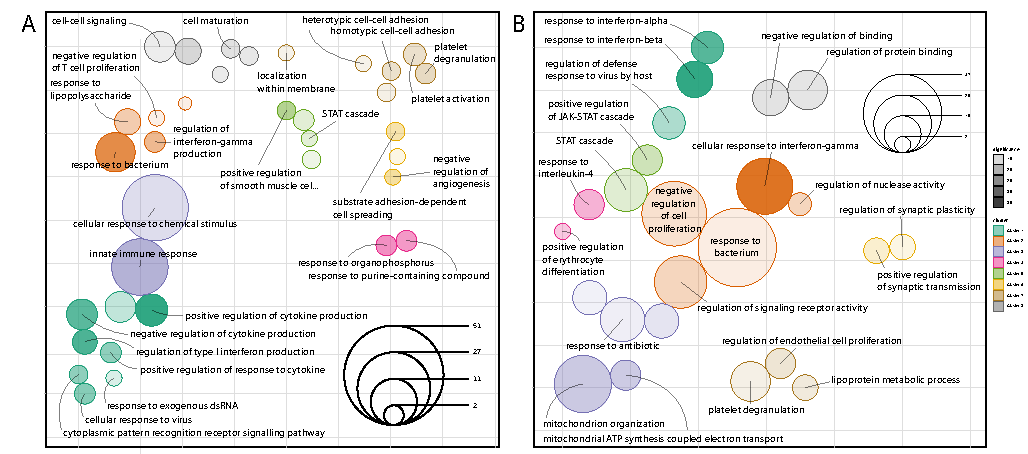
\includegraphics[width=\textwidth]{figures/gsoap-de}
\caption[Large RNA Differential Expression Gene Ontology Enrichment.]{\textbf{Large RNA Differential Expression Gene Ontology Enrichment.} GO terms from enrichment analysis were projected on a 2D map via \acf{tsne} analysis of their shared significant genes. LEGEND \textbf{A)} \ac{tsne} visualisation of GO terms of DE genes with \ac{lfc} > 1.4 shows 36 terms in eight clusters. Immunological terms (left-hand side) and circulatory terms (right-hand side) are predominant. \textbf{B)} \ac{tsne} visualisation of 24 GO terms of top 100 genes measured by count-change corroborate immunological changes in stroke patient blood differential gene expression.
\label{fig:gsoap-de}}
\end{figure}

As a cross-check, \ac{de} transcripts were ranked by count-change, and re-analysed (Figure \ref{fig:gsoap-de}\,B). The top 100 changed transcripts, without regard to direction (absolute count-change) yielded terms implying response to \ac{ifn} $\upalpha$ (\e{3.8}{-4}), $\upbeta$ (\e{1.1}{-4}), and $\upgamma$ (\e{1.4}{-4}), mitochondrial organisation (\e{5.6}{-3}) and ATP synthesis (\e{6.9}{-3}), response to \ac{il}-4 (\e{6.9}{-3}), positive regulation of JAK-STAT cascade (\e{8.8}{-3}), response to antibiotic (0.044), and platelet degranulation (0.045). The top 100 up-regu"-la"-ted transcripts yielded terms involving platelet degranulation (\e{3.8}{-3}), mitochondrial ATP synthesis (\e{4.2}{-3}), response to xenobiotic stimulus (0.017), platelet aggregation (0.013), and response to antibiotic (0.016), while the top 100 down-regulated transcripts were associated with inflammatory response (\e{1.3}{-4}), regulation of apoptosis (\e{1.8}{-4}), cytokine secretion (\e{6.8}{-4}), antigen processing and presentation (\e{1.2}{-3}), regulation of lymphocyte apoptosis (\e{2.3}{-3}) and proliferation (\e{2.7}{-3}), response to antibiotic (\e{5.2}{-3}), leukocyte homeostasis (\e{7.6}{-3}), response to \ac{il}-1 (\e{7.6}{-3}), and many more immune-specific processes. This corroborates the previous findings that up-regulated transcripts represent the response to circulatory system damage, and down-regulated transcripts indicate a cytokine-mediated immunodepression. For a full list of all terms from these analyses\todo{DE genes?}, see Appendix \ref{appendix:go-terms-large-rna}. 

\subsection{Differential Expression of small RNA}
In the simultaneous co-analysis of miRNAs and tRFs, we detected 420 DE miRNAs and 143 DE tRFs (adjusted p-value < 0.05, Figure \ref{fig:stroke-de-tsne}\,B\&C). 63\% of miRNAs (265) were down-regulated, while 87\% of tRFs (124) were up-regulated. tRFs were mainly derived from the 3' end (3'-tRFs, 87) or from internal tRNA regions (i-tRFs, 48), while the tRFs from 5' ends (5'-tRFs) were in the minority (6). The amino acid distribution was shifted in favour of alanine- (35), glycine- (28), and proline-carrying (12) tRNAs (Figure \ref{fig:stroke-de-tsne}\,D). 30 of the 35 alanine-associated tRFs were 3'-tRFs, and all of those were up-regulated, indicating non-random generation of these fragments.

\begin{figure}[ht]
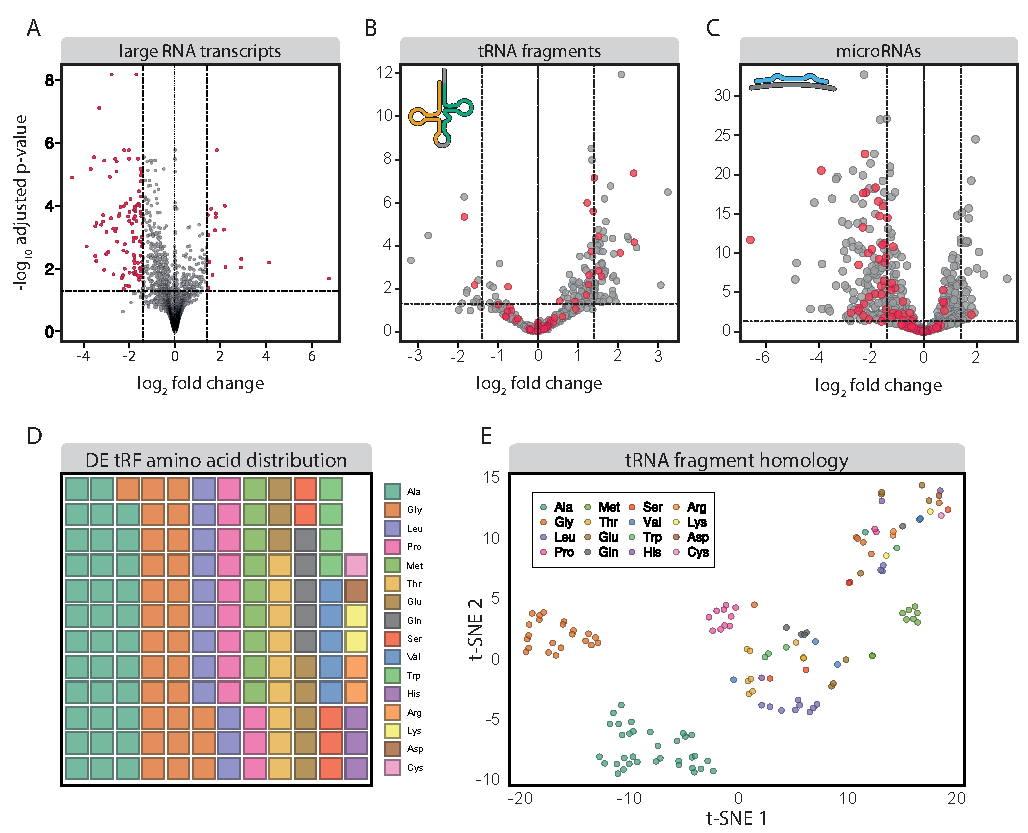
\includegraphics[width=\textwidth]{figures/stroke-de-tsne}
\caption[Small and Large RNA Differential Expression and tRF Properties.]{\textbf{Small and Large RNA Differential Expression and tRF Properties.} \textbf{A)} Differential expression analysis reveals multiple large RNA transcripts changed in patient blood after stroke. The majority of differentially expressed (DE) transcripts above a \ac{lfc} threshold of 1.4 (red) are down-regulated. \textbf{B)} Blood-borne tRNA fragments (tRFs) also change after stroke. Unlike large RNA and miRNAs, the majority of DE tRFs are up-regulated. \Acf{ca} tRFs in red. \textbf{C)} Blood-borne miRNAs are heavily influenced by the events following stroke. Like large RNA transcripts, miRNAs are also overwhelmingly down-regulated. \Ac{ca} miRNAs in red. \textbf{D)} The distribution of amino acid origin among the DE tRFs is non-random and biased towards the amino acids alanine, glycine, leucine, proline, and methionine. Each square represents one DE tRF, colour denotes amino acid origin. \textbf{E)} \acf{tsne} of pairwise fragment homology by local Smith-Waterman alignment shows clustering of the dominant amino acid groups of tRFs. Clear clusters can be observed for tRFs derived from tRNA carrying alanine, glycine, leucine, proline, and methionine.
\label{fig:stroke-de-tsne}}
\end{figure}

\subsection{Homology Among tRNA Fragments}
Using pairwise homology among all DE tRFs, visualised via \ac{tsne} (see Section \ref{sec:stroke:tsne}), we identified clusters of highly similar fragments, that correlate with their amino-acid origin, i.e., the amino acid which is carried by the respective parent tRNA (Figure \ref{fig:stroke-de-tsne}\,E). This relationship persisted across distinct individual tRNAs coding for the same amino acid, and was particularly pronounced in tRNAs associated with alanine, glycine, leucine, proline, and methionine. This further indication of non-random generation of tRNA fragments shorter than tiRNAs leaves an open question about their biogenesis, particularly, which nucleases are responsible for the generation of the mature transcripts, and if 3'-tRF generation is dependent or independent from tiRNA generation by angiogenin.

\subsection{Cholinergic Association of Small RNA Species}
The association of smRNA species to distinct systems or pathways is not trivial because of the multiple-targeting nature of these RNAs. For the purpose of the following analyses, we defined a small RNA as being associated with cholinergic processes by the positive association of the smRNA with a number of \acf{ca} large transcripts. We do not assess the question whether this small RNA also targets other systems equally, or even if it targets cholinergic transcripts with greater likelihood than a random selection of genes. For this reason, we select a fairly high threshold for the definition of a \ac{ca} smRNA, which is the targeting of at least 5 \ac{ca} transcripts (above 80\% on the empirical cumulative density function of cholinergic targeting, see Section \ref{sec:stroke:chol-assoc}).

Following this definition, we detected 52 \ac{ca} miRNAs (90\% down-regulated, 5 up and 47 down), and 18 \ac{ca} tRFs (83\% up-regulated, 15 up and 3 down). Above an \ac{lfc} threshold of 1.4, we found 33 \ac{ca} miRNAs (97\% down-regulated, 1 up and 32 down), and 9 \ac{ca} tRFs (78\% up-regulated, 7 up and 2 down). \ac{ca} smRNAs are marked in red in Figure \ref{fig:stroke-de-tsne}\,B\&C.\todo{amino acids?}

\newpage

%!TEX root = ../dissertation.tex
\section[Blood Compartments of Cholinergic Systems and Small RNA Species]{Blood Compartments of Cholinergic Systems \\and Small RNA Species} \label{sec:stroke:celltypes}
To address the shortcomings of whole-blood RNA sequencing, which is more representative of the clinical setting, but less specific regarding cellular compartments, we consulted third party datasets to assess RNA species distribution in different cellular and non-cellular compartments of the blood. For small RNA species, we re-analysed a published dataset of small \ac{seq} of 450 human samples from various blood tissues;\cite{Juzenas2017} for large RNA transcripts, we utilised the tissue specificity of Marbach's regulatory circuits.\cite{Marbach2016} The large RNA information was used to identify blood cell types with cholinergic transcriptional activity, which was then used to zoom in into small RNA expression subsets related to cholinergic processes.

\begin{method}

\subsection{Large RNA Regulatory Circuits in Tissues of the Blood}
To evaluate the cell type distribution of cholinergic genes in blood tissue types, we utilised the expression patterns derived from cumulative transcription factor activity of Marbach's regulatory circuits.\cite{Marbach2016} As shown by the authors, the cumulative activity of all transcription factors towards one gene describe well the actual expression of that gene in the respective tissue type. To maximise comparability to the parallel analyses of small RNA species (Section \ref{sec:stroke:juzenas}), blood cell types (i.e., »regulatory circuits«) were selected to reflect the cell type selection of Juzenas \emph{et al.}\cite{Juzenas2017} based on similar markers of the »cluster of differentiation« family of genes. These were: CD4$^+$ T-helper cells, CD8$^+$ cytotoxic T-cells, CD14$^+$ monocytes, CD15$^+$ neutrophils, CD19$^+$ B-cells, CD56$^+$ natural killer cells, and, for comparison, whole blood. For the sake of simplicity, genes were considered »present« in each blood tissue type if at least one TF showed significant activity towards the gene.

TF activities were collected for all of the tissues and aggregated across all TFs per gene by summing. The resulting table of 15\,032 genes in the seven tissues was used as input for the \emph{Rtsne} function.\cite{Krijthe2015} t-SNE was computed using a range of perplexities and visualised as 2D map with a perplexity of 49 using R/ggplot2.\cite{Wickham2016}

\subsection{An Atlas of Small RNA Expression in Cell Types of the Blood} \label{sec:stroke:juzenas}
To evaluate the cell type distribution of our small RNA molecules, we analysed a dataset deposited by Juzenas \emph{et al.},\cite{Juzenas2017} who separated and sequenced 450 samples comprising seven types of individual blood cell types (characterised by »cluster of differentiation«-type membrane-bound receptors), serum, exosomes, and whole blood (Figure \ref{fig:celltype-presence}\,A). The individual blood cell types comprised CD4$^+$ T-helper cells, CD8$^+$ cytotoxic T-cells, CD14$^+$ monocytes, CD15$^+$ neutrophils, CD19$^+$ B-cells, CD56$^+$ natural killer cells, and CD235a$^+$ erythrocytes (the only distinct cell type not available in Marbach's regulatory circuits, since mature erythrocytes do not transcribe). Starting from the raw data deposited on NCBI GEO, we controlled the quality, applied quality-based filtering, and aligned the 450 samples to miRNA and tRF sequences, as described in Section \ref{sec:stroke:alignment}. The original publication did not offer statistical analyses because of a failure in the spike-in procedure, and defined presence of a small RNA by a measure of at least five counts in 85\% of samples. However, since this definition relies heavily on sequencing depth, and depth can vary widely even in methodically robust sequencing experiments depending on a large number of variables (see Figure \ref{fig:read-quality-length}\,C), we defined our own test for descriptive analysis of presence or absence of lowly expressed small RNAs in each of the sample types (Section \ref{sec:stroke:presence}).

\begin{figure}
\centering
\includegraphics[width=.7\textwidth]{figures/celltype-presence}
\caption[Small RNA Sequencing of Sorted Cell Types of the Blood and Definition of Presence/Absence.]{\textbf{Small RNA Sequencing of Sorted Cell Types of the Blood and Definition of Presence/Absence.} \textbf{A)} Data deposited by Juzenas \emph{et al.}\cite{Juzenas2017} include smRNA-information on CD4$^+$ T-helper cells, CD8$^+$ cytotoxic T-cells, CD14$^+$ monocytes, CD15$^+$ neutrophils, CD19$^+$ B-cells, CD56$^+$ natural killer cells, CD235a$^+$ erythrocytes, serum, exosomes, and whole blood. Raw data were re-analysed to yield miRNA- and tRF-expression levels. \textbf{B)} Definition of presence or absence of small RNA molecules from RNA-sequencing data is based on log-normality of count data, irrespective of expression levels. Log-normal distributions were calculated using the mean and standard deviation of expression levels (green lines) and compared to the actual distribution via the Kolmogorov-Smirnov test. Presence (upper example) was assumed at a relatively stringent level of p > 0.1. The red line indicates a power-law distribution in comparison (absence, lower example).
\label{fig:celltype-presence}}
\end{figure}

\subsection[Definition of Presence and Absence of Lowly Expressed\texorpdfstring{\\}{} smRNA Molecules]{Definition of Presence and Absence of Lowly Expressed smRNA Molecules} \label{sec:stroke:presence}
This definition comprises estimation of a log-normal distribution from a small RNA expression profile, and a statistical test to refute the null hypothesis that the distribution is in fact log-normal. The danger of evaluating true expression of lowly expressed smRNA molecules by a count-based threshold is the possibility of random reads resulting from degradation products of highly expressed RNA with similar sequence, and the amplification of noise. Both problems are exacerbated by an increase in sequencing depth. In today's \ac{seq} technology, most chips can accommodate only a limited amount of samples compared to the amount of reads that can be generated. While this is not as problematic in cases of longer inserts and paired design, which is usually employed in large \ac{seq}, in small \ac{seq} this can lead to enormous overheads of reads. It is not uncommon to receive tens of millions of reads for each sample, which exceeds the recommended amount (of at least one million) by large margins.

Thus, there is the need to distinguish between degradation products of highly expressed RNA molecules or amplified noise and legitimate lowly expressed smRNA molecules (even more so since one of the smRNA species is a product of non-random tRNA degradation). The central assumption for our proposed method is: The expression pattern of legitimate smRNA molecules follows, as is common in biology, a normal distribution of some kind, or, for the discrete case, a normal poisson distribution. On the other hand, degradation products or noise would rather follow other, »non-biological« distributions, such as a uniform distribution or a monotonously decreasing power-law distribution such as the Pareto distribution. Thus, we chose to statistically test each smRNA in each tissue type for the adherence to this criterion, by comparing the measured counts with a distribution function estimated based on the mean and standard deviation of the measured counts. During testing, we found the log-normal distribution to give the best classification results.
 
The distribution mean and standard deviation of the expression values per cell type and smRNA were estimated using the \emph{fitdist} function of the R/fitdistrplus package.\cite{Delignette-Muller2015} The count distribution was then tested against a log-normal distribution with the estimated mean and standard deviation via the R implementation of the Kolmogorov\=/Smirnov test, with a cutoff of 0.1. The small RNA was defined as present if the test failed to reject the null hypothesis (Figure \ref{fig:celltype-presence}\,B).

\subsubsection{Analysis of Expression Patterns and Establishment of Virtual Tissues}
The distribution of smRNA expression across the different cell types was used to assign eight functional compartments (i.e., »virtual tissues«) to the entirety of detected fragments such that each smRNA was sorted into one of the tissue classes. Ideally, these classes would be unambiguous, i.e., there would be no overlap of smRNA molecules between the classes. Eight classes were created via hierarchical clustering of miRNA and tRF expression separately (Figure \ref{fig:heatmaps-small}), and then used in combination with t-SNE applied to the entire expression matrix, to visualise the compartmentalisation of smRNAs in these virtual tissues. The samples taken from stroke patients in the PREDICT study were sequenced from whole blood, which precludes direct information about tissue distribution. Thus, the two-dimensional maps from t-SNE visualisation were used to, first, explore the tissue association of smRNAs differentially expressed in whole blood samples of stroke patients, and second, examine the potential impact of \acl{ca} smRNAs in these tissues.

\end{method}

\begin{figure}[ht]
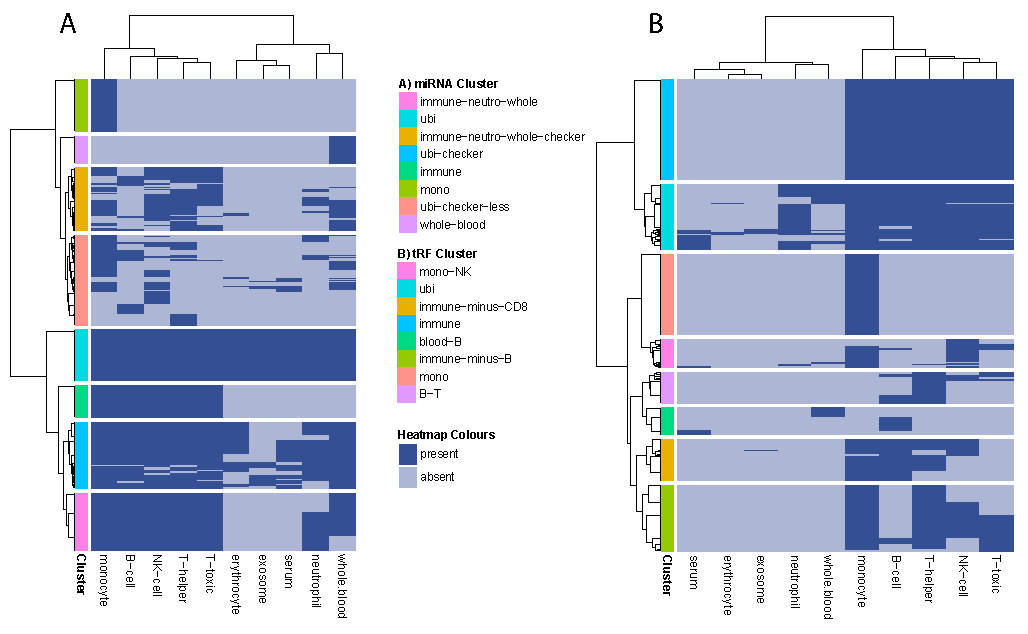
\includegraphics[width=\textwidth]{figures/heatmaps-small}
\caption[Functional Characterisation of Hierarchical Clusters in Blood Cell Small RNA Expression.]{\textbf{Functional Characterisation of Hierarchical Clusters in Blood Cell Small RNA Expression.} Information on presence/absence of miRNAs and tRFs in the tissue types analysed in Juzenas \emph{et al.}\cite{Juzenas2017} were hierarchically clustered into 8 clusters using the Ward method,\cite{Ward1963} and plotted on a heatmap (single smRNAs on the y-axis, tissue types on the x-axis). To assign meaning to these clusters, manual inspection was followed by annotation of enrichment in tissue types. Complex combinations were approximated by their most prominent features. \textbf{A)} Clusters of miRNA presence/absence in blood cell compartments. Clearest cluster association was shown by miRNAs expressed only in monocytes (»mono«), in all blood-borne immune cells except neutrophils (»immune«), ubiquitously without exception (»ubi«), and only in whole blood (i.e., in none of the single compartments (»whole-blood«). \textbf{B)} Clusters of tRF presence/absence in blood cell compartments. Clearest cluster association was shown by tRFs expressed only in monocytes (»mono«), and in all blood-borne immune cells except neutrophils (»immune«). The other tissue-related clusters were not as clear as in the miRNA expression data, indicating a looser association to cell type of tRNA-derived smRNAs.
\label{fig:heatmaps-small}}
\end{figure}

\subsection{Large RNA Expression Patterns Identify Cholinergic Systems\\ in CD14$^+$ Monocytes}
The expression patterns of 15\,032 large RNA molecules in blood-borne immune cells were visualised in a t-SNE-derived 2D map (Figure \ref{fig:tsne-large}\,A). More than half of all transcripts show highest expression in whole blood (7533, not shown), so subsequent analyses were performed on the set of six tissues, without the whole blood compartment. In this set (14\,280 genes), most transcripts show highest expression in CD14$^+$ monocytes (9125 transcripts), followed by CD19$^+$ B-cells (1176) and CD15$^+$ neutrophils (1166). Remaining are CD4$^+$ T-helper cells (1092), CD56$^+$ NK-cells (948), and CD8$^+$ cytotoxic T-cells (773). When filtered for cholinergic genes, there is visible enrichment of core cholinergic transcripts in a spatial sub-compartment of CD14$^+$ monocytes (Figure \ref{fig:tsne-large}\,B). Considering the different monocyte phenotypes (pro- and anti-inflam"-ma"-to"-ry, see Section \ref{sec:intro:stroke}), and their implied transcriptomic differences, which most likely are brought on by divergent TF activity, this compartmentalisation of cholinergic transcripts inside one spatial sub-compartment may indicate a cholinergic »preference« in favour of one particular monocyte phenotype. 

\begin{figure}
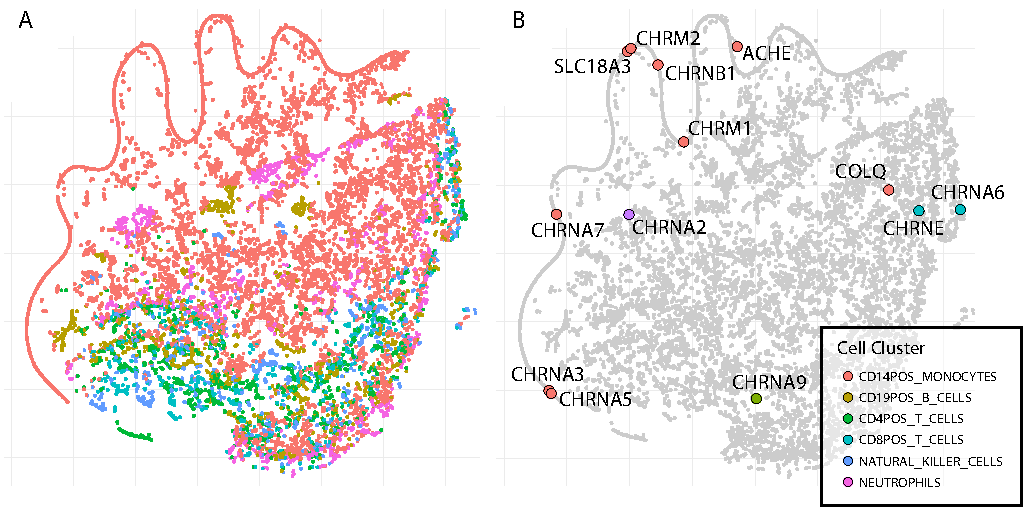
\includegraphics[width=\textwidth]{figures/tsne-large}
\caption[Large RNA Expression Patterns in Blood-Borne Cells.]{\textbf{Large RNA Expression Patterns in Blood-Borne Cells.} Expression derived from transcriptional activity in blood-borne cell types in the Marbach dataset\cite{Marbach2016} was visualised via t-SNE. The input matrix comprised all 14\,280 detected genes in 6 types of blood-borne immune cells. Genes were plotted on the first two t-SNE dimensions and coloured by the cell type of their highest expression, i.e., the highest cumulative transcriptional activity of all active TFs. \textbf{A)} Complete t-SNE shows a gradient of expression across the different cell types, with much expression in CD14$^+$ monocytes and T-cells. \textbf{B)} Highlighting of cholinergic core genes reveals an enrichment in close compartments of CD14$^+$ monocytes. The vesicular ACh-transporter SLC18A3 can serve as substitute for the main cholinergic marker, CHAT, as discussed in Section \ref{sec:database:tf}.
\label{fig:tsne-large}}
\end{figure}

\subsection{Identification of Functional Enrichment of \\smRNA Expression in Blood-Borne Cells}
To date, there is no comprehensive expression catalogue of smRNA species expression in the tissue types of the human body that is comparable to what has been achieved in the description of large RNA. To classify the detected smRNAs in a manner specific to tissues in human blood, we utilised a dataset published by Juzenas \emph{et al.},\cite{Juzenas2017} who describe miRNA expression in a variety of blood tissues. We re-analysed the publicly deposited data for miRNA and tRF expression, and developed our own method of defining »presence« of the smRNA in each tissue type based on the evaluation of a log-normal distribution model (instead of using a simple count threshold, see Section \ref{sec:stroke:juzenas} for details). 

Using these presence/absence data, we first utilised hierarchical clustering to establish »virtual tissues« that could be assigned to each smRNA (Figure \ref{fig:heatmaps-small}) for later evaluation in the stroke patient sequencing. Both miRNAs as well as tRFs showed a number of smRNAs clearly associated with several compartments, whereas other compartments and smRNAs were distributed in a more complex manner. The ten tissue types of the Juzenas \emph{et al.}\cite{Juzenas2017} study were equally parted into two five-tissue superclusters by the expression patterns of both smRNA species (Figures \ref{fig:heatmaps-small}\,A\&B, x-axis). These two clusters distinguish immune from non-immune compartments in the blood, but for one notable exception: while the »immune supercluster« comprises monocytes, T-cells, B-cells, and NK-cells, the »non-immune supercluster« contains neutrophils in addition to erythrocytes and the non-cellular tissues serum, exosomes, and whole blood. Notably, the neutrophil samples cluster closest to the whole blood compartment in both smRNA species.

Two distinct virtual tissues showed high consistency in both smRNA species: a virtual tissue containing only CD14$^+$ monocytes and another tissue comprising all studied cellular immune components except neutrophils (i.e., monocytes, B-cells, both types of T-cells, and NK-cells). miRNAs (Figure \ref{fig:heatmaps-small}\,A), in addition, yield clear clusters for miRNAs expressed in whole blood, and for miRNAs expressed ubiquitously without exception. In tRFs (Figure \ref{fig:heatmaps-small}\,B), the general picture is more complex, as the clusters are often mixed.

\subsection{Expression Patterns of Differentially Expressed and\\ Cholinergic-Associated smRNAs}
Similarly to the visualisation of large RNA molecules, the expression patterns of 600 miRNAs and 1671 tRFs in ten tissues of the blood were visualised in t-SNE-derived 2D maps (Figure \ref{fig:tsne-small}\,A\&B). In the initial visualisation, the forming of multiple clusters according to some virtual tissues can be observed, while other virtual tissues are visibly more dispersed. Clearest clusters are formed in both cases by ubiquitously expressed smRNAs (»ubi«), smRNAs expressed only in monocytes (»mono«), and smRNAs equally expressed in all immune-related blood-borne cells except for neutrophils (»immune«). Examination of DE smRNAs on this 2D map shows a further parallel between miRNAs and tRFs (Figure \ref{fig:tsne-small}\,C\&D): differential expression after stroke takes place in all compartments of the blood, and highest changes in transcript amount (as measured by count-change) are observed in ubiquitously expressed smRNAs. Similarly, \acf{ca} miRNAs and tRFs (Figure \ref{fig:tsne-small}\,E\&F) are observed in all compartments, but the most highly differentially regulated CA smRNAs are expressed in all blood compartments alike. Notably, whole blood does not play a role in DE miRNAs, which may indicate lower relative importance of non-cellular blood compartments in terms of classification. In other words, most smRNAs that are found in non-cellular compartments are found in the cellular compartments as well, making them irrelevant for classification (however, their biological function in these non-cellular compartments remains a matter of interest).

\begin{figure}
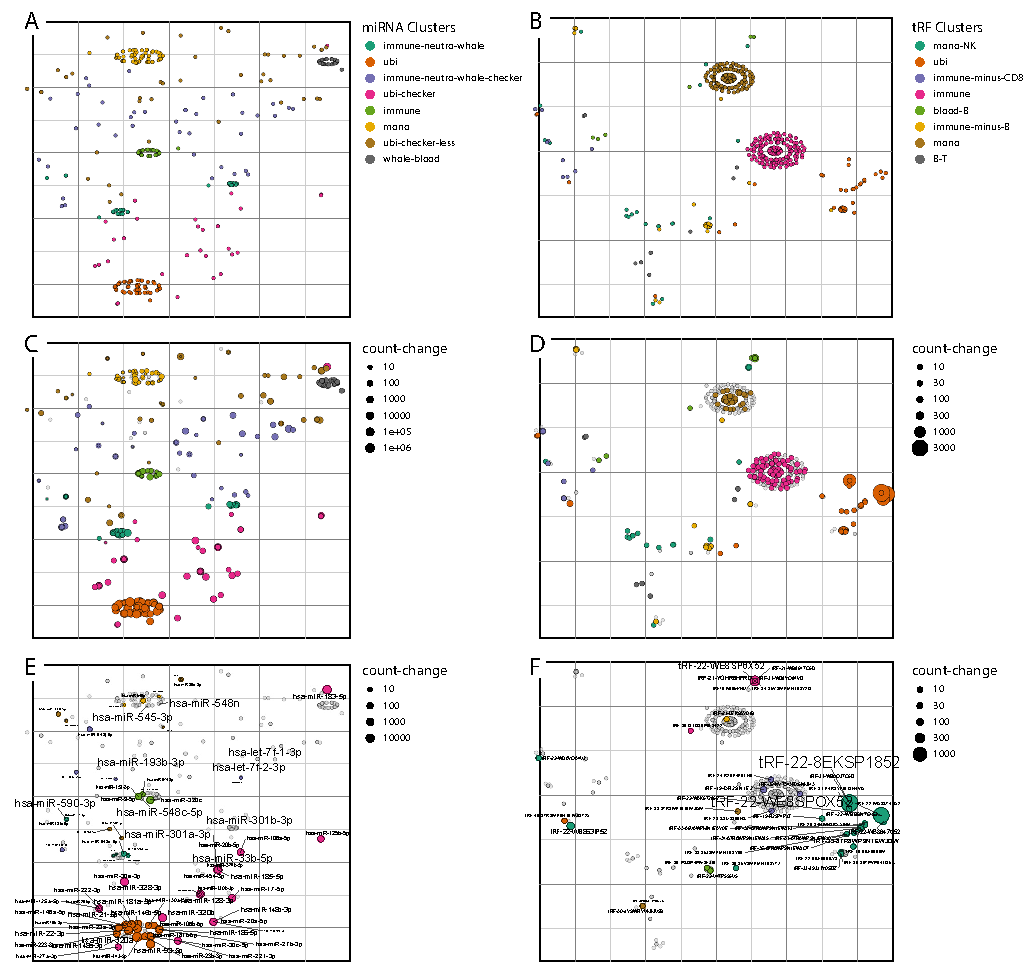
\includegraphics[width=\textwidth]{figures/tsne-small}
\caption[Small RNA Expression Patterns in Blood-Borne Cells.]{\textbf{Small RNA Expression Patterns in Blood-Borne Cells.} Two-dimensional expression maps were created using t-SNE on the full numeric expression data derived from re-analysis of the Juzenas \emph{et al.}\cite{Juzenas2017} data set for miRNAs and tRFs separately. Single smRNAs (points) were coloured by the virtual tissues derived from the cluster heatmap analysis (Figure \ref{fig:heatmaps-small}). Node size reflects absolute count change in \textbf{C}, \textbf{D}, \textbf{E}, and \textbf{F}. Shown are full data, differentially expressed (DE) smRNAs, and \acf{ca} smRNAs for each species. \textbf{A)} Full t-SNE visualisation of miRNA expression. The largest 2D-associative clusters are comprised of the clearest presence/absence virtual tissues, monocytes (yellow) and ubiquitously expressed (orange). Smaller clusters can be identified for the tissue of all immune cells except neutrophils (green) and the complex cluster of immune cells including neutrophils and whole blood (turquoise). \textbf{B)} Full t-SNE visualisation of tRF expression. The largest 2D-associative clusters are, as in miRNAs, comprised of the clearest presence/absence virtual tissues, monocytes (brown) and immune cells except neutrophils (pink). A smaller cluster can be identified for ubiquitously expressed tRFs (orange). \textbf{C)} miRNAs \ac{de} after stroke are ubiquitously expressed in all virtual tissues. Highest differential expression is seen in the »ubi« cluster. \textbf{D)} Likewise, tRFs \ac{de} after stroke are ubiquitously expressed in all virtual tissues, and highest differential expression is seen in the »ubi« cluster. \textbf{E)} \Ac{ca} miRNAs are enriched in the lower quadrants of the 2D map, particularly in the clusters associated with ubiquitous expression (»ubi«, »ubi-checker«). \textbf{F)} \Ac{ca} tRFs show a similar distribution, skewed towards virtual tissues with ubiquitous expression. This may indicate covariation of detection with broadness of expression (see text and Section \ref{sec:discussion:stroke-blood}).
\label{fig:tsne-small}}
\end{figure}

On the other hand, smRNAs that are ubiquitously expressed are also detected in differential expression with high frequency and perturbation (see Figure \ref{fig:tsne-small}\,C\&D). In addition to a putatively significant biological function of these smRNAs, this may also indicate a covariation of broadness of expression with detection in whole blood differential expression. Presenting an important limitation, this possibility cannot be assessed in the present data, because it requires a stratification of blood tissues prior to sequencing, for instance via fluorescence-assisted or magnetic-activated cell sorting (FACS/MACS). This issue is further discussed in Section \ref{sec:discussion:stroke-blood}.

%\newpage

\section[Regulatory Circuits of Small RNA and Transcription Factors in CD14$^+$ Monocytes]{Regulatory Circuits of Small RNA and \\Transcription Factors in CD14$^+$ Monocytes}
The clear separation of CD14$^+$-biased smRNAs (Figure \ref{fig:heatmaps-small}) and the cholinergic importance of CD14$^+$ monocytes as shown by large RNA t-SNE (Figure \ref{fig:tsne-large}) merit a detailed analysis of these cells in terms of their transcriptomic interactions. We thus created the whole-transcriptome network of transcription factors, miRNAs, tRFs, and target genes in CD14$^+$ monocytes using \emph{miRNeo}, and analysed it in different ways.

\begin{method}

\subsection{Comprehensive Circuit Network Creation} \label{sec:stroke:circuit-network}
The comprehensive transcriptomic network in CD14$^+$ monocytes was created in a two-step process of \emph{miRNeo} targeting. First, the complete TF$\to$gene network was created from the targeting data derived from Marbach \emph{et al.}\cite{Marbach2016}, yielding a CD14-specific network comprising 616 TFs with activity towards 13\,447 transcripts, in 318\,731 unique interactions. Second, this network was then subjected to successive \emph{miRNeo} targeting of all transcripts in the network by miRNAs and tRFs.

For each node fulfilling an active role in this network (i.e., miRNAs, tRFs, and TFs), an activity parameter was computed. The activity of each node is hereby defined as the sum of all scores of each of its targeting relationships. In the case of miRNAs, the score is the summary score introduced in Section \ref{sec:database:mirna}; for tRFs, it is the score calculated with the BL-PCT method (see Section \ref{sec:database:trf-targeting}); and for TFs, it is the transcriptional activity given by Marbach and colleagues.\cite{Marbach2016} Activities were normalised, for each biotype separately, by scaling the calculated values $v$ onto a range between 0 and 1, using $$v_{i, norm} = \frac{v_i}{max(v)}$$
with $max(v)$ being the maximum of all scores in this biotype category, and all $v$ > 0. The activity of each relationship determined the weight of the edge between the two connected nodes.

The network was visualised in gephi,\cite{Jacomy2014} omitting all non-TF genes, and using ForceAtlas2 to generate a force-directed 2D map of smRNA$\to$TF interactions in CD14$^+$ monocytes. Network modularity was calculated using the function included in gephi,\cite{Blondel2008} with a resolution of 2.0, to yield two distinct modularity classes of predominant regulation by either miRNAs or tRFs. The associations of TFs to the tRF- and miRNA-regulated modules were used to perform subsequent analyses of the distinct modules. 

\subsection[Gene Ontology Analyses of TF$\to$Gene Networks\texorpdfstring{\\}{} of CD14$^+$ Monocytes]{Gene Ontology Analyses of TF$\to$Gene Networks of CD14$^+$ Monocytes} \label{sec:stroke:go-cd14}
The TF$\to$gene networks of each of the two modules derived from smRNA species association (miRNAs versus tRFs) were analysed using topGO\cite{Alexa2006} essentially as described in Section \ref{sec:cellculture:topgo}. Genes were ordered according to the cumulative activity of TF targeting of each gene in CD14$^+$ monocytes. To display a range of top genes, transcript background was iterated in five equal steps from 1000 transcripts to the maximum size of target transcripts in each network (12\,927 for miRNA-targeted TFs, 12\,904 for tRF-targeted TFs). The test set was the top 10\% of transcripts for each background size. GO terms were collected and screened for multiple entries among the sets. The most prevalent terms were used to infer the functional roles of miRNA- and tRF-targeted transcription factors. We determined the overlap of GO terms between both smRNA species as well as the terms exclusive to either. 

\end{method}

\subsection{Dichotomy of Small RNA Targeting of \\Transcription Factors in CD14$^+$ Monocytes}
Organisation of the smRNA$\to$TF network via a force-directed algorithm resulted in visible clustering of two distinct subnetworks, that are governed by miRNAs and tRFs, respectively (Figure \ref{fig:smrna-tf-network-fractions}). Inside this network, 10 TFs were found DE in patient blood after stroke (Figure \ref{fig:smrna-tf-network-fractions}\,A). Calculation of modularity clearly divided the network into TFs primarily influenced by miRNAs and TFs primarily influenced by tRFs (Figure \ref{fig:smrna-tf-network-fractions}\,B). Based on these two sets of TFs, two distinct TF$\to$gene networks were created: 289 miRNA-biased TFs with 152\,649 unique TF$\to$gene targeting relationships, and 280 tRF-biased TFs with 163\,641 unique TF$\to$gene targeting relationships.

\subsection{Gradual Shift in Control Over Transcription Factors\\ by miRNAs and tRFs}
356 TFs were detected in the stroke patient blood sequencing experiment. It is notable that, although the complete graph shows clear segregation between miRNA-targeted and tRF-targeted transcripts, merely 106 of those TFs are targeted by only one of the two smRNA species (48 only by miRNAs and 58 only by tRFs), and 55 are supposedly not at all targeted by any smRNA present in CD14$^+$ cells. The remaining 195 TFs are putative targets of both smRNA species (Figure \ref{fig:smrna-tf-network-fractions}\,C). 

At an alpha level of 0.1 for the differential expression between stroke patients and controls, 26 of these TFs remain, also showing a gradual pattern of targeting by miRNAs and tRFs (Figure \ref{fig:smrna-tf-network-fractions}\,D). Six of these transcription factors are implicated in the control of cholinergic core or receptor genes (marked with a »C«). It is notable that a number of TFs show no indication of being a target of either smRNA species present in CD14$^+$ cells under the premises of our targeting approach (Figure \ref{fig:smrna-tf-network-fractions}\,E). Considering the multiple-targeting behaviour of smRNAs, and the general experience that non-targeted genes are uncommon, this finding is interesting in itself, particularly since it involves well-described regulators of immunological processes, such as \emph{STAT2} and \emph{ELF1}.

\begin{figure}
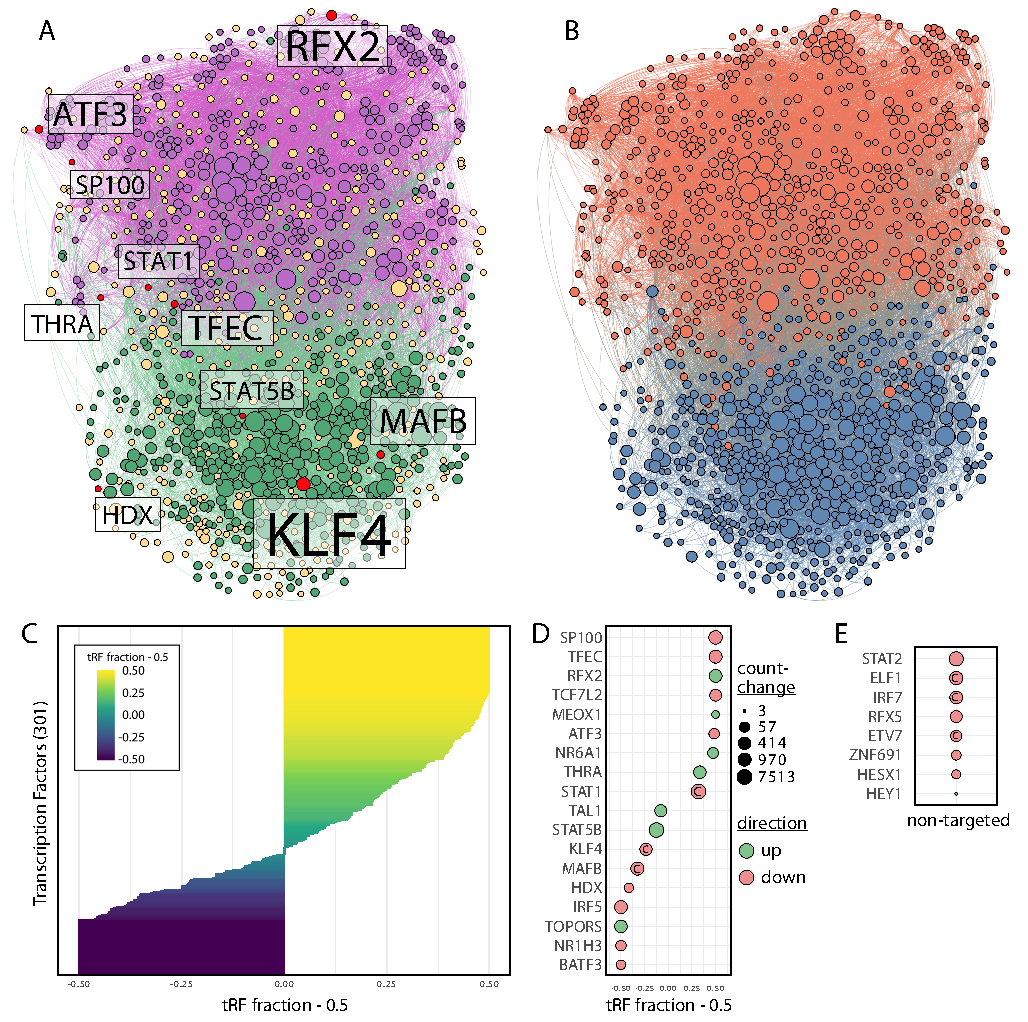
\includegraphics[width=\textwidth]{figures/smrna-tf-network-fractions}
\caption[Small RNA Targeting of Transcription Factors in CD14$^+$ Monocytes.]{\textbf{Small RNA Targeting of Transcription Factors in CD14$^+$ Monocytes.} The two-dimensional map of all TFs active in CD14$^+$ monocytes and their smRNA controllers was created via \emph{miRNeo} targeting and visualisation via force-directed algorithm. Node size is determined by activity (see Section \ref{sec:stroke:circuit-network}). \textbf{A)} Nodes coloured by biotype: miRNAs - green, tRFs - purple, TFs - yellow, differentially expressed (DE) TFs - red. TFs targeted mainly by tRFs segregate visually from TFs targeted mainly by miRNAs. Both sets contain DE TFs, indicating complementary function. \textbf{B)} The network was divided into two modules by network connectivity measures. Node colour denotes modularity class association. Network modularity largely reflects TF targeting of tRFs (orange) versus miRNAs (blue). \textbf{C)} Bar graph displays the fraction of smRNAs of each species targeting each of the TFs (on the y-axis, 301 TFs). A tRF fraction of 1 means all smRNAs targeting the TF are tRFs, 0 means all are miRNAs. Displayed on x axis is »tRF fraction - 0.5« to center on 50:50 targeting by both species. 48 TFs are solely targeted by miRNAs (leftmost) and 58 solely by tRFs (rightmost). \textbf{D)} Similarly, TFs differentially expressed in the blood of stroke victims show a distribution on the miRNA-tRF gradient. Point size denotes count-change, point colour denotes direction of change; a »C« denotes the TF as targeting cholinergic core and receptor genes. \textbf{E)} Notably, there is also a set of TFs that are supposedly not targeted by any smRNA present in CD14$^+$ cells.
\label{fig:smrna-tf-network-fractions}}
\end{figure}

The \emph{STAT} family of transcription factors is an interesting example in this analysis. The cholinergic/neurokine interface is facilitated by JAK/STAT signalling, in which neurokine receptors can activate the pathway through STAT1, STAT3, and STAT5A/B phosphorylation.\cite{Lobentanzer2019a} There are three differentially expressed STATs in our data set: STAT1 is down-regulated (highest absolute count-change of all TFs), targeted preferentially by tRFs (tRF fraction = 82.1\%), and directly associated with cholinergic genes in CD14$^+$ monocytes (»C«); STAT5B is up-regulated (second highest count-change of all TFs), preferentially targeted by miRNAs (tRF fraction = 37.5\%), and not directly associated with cholinergic genes in CD14$^+$ cells; and STAT2 is also down-regulated (third highest absolute count-change of all TFs), does not directly associate with cholinergic genes, and additionally is not predicted to be targeted by any smRNA present in CD14$^+$ monocytes, although it is expressed and induced by interferons in these cells.\cite{Lehtonen1997} 

\subsection{Dichotomous Transcriptomic Footprints of \\Transcription Factors in CD14$^+$ Monocytes}
To determine the putative effect of TF regulation by each smRNA species, we evaluated the potential impact of the TFs most targeted by either miRNAs or tRFs (i.e., the two modules from Figure \ref{fig:smrna-tf-network-fractions}\,B). The top 10\% of TF targets in CD14$^+$ monocytes (derived from Marbach \emph{et al.}\cite{Marbach2016}) were subjected to iterative GO analysis (see Section \ref{sec:stroke:go-cd14}). Assuming a general effect of repression in tRF-targeted TFs (because the majority of DE tRFs are up-regulated), and a general de-repression in the set of miRNA-targeted TFs (because most DE miRNAs are down-regulated), the putative functional effects of changes in smRNA levels can be described by GO enrichment analysis of these two test sets. Although this is a very rough categorisation, it may help in classifying the areas of influence shared between the two smRNA species, or exclusive to either.

\subsubsection{GO Term Overlap Between miRNA- and tRF-targeted \\Transcription Factors}
If we assume the functions associated with TF$\to$gene interaction (the »footprint«) in each subnetwork under miRNA or tRF control as an indication of the sphere of (most) influence of this smRNA species, the GO terms associated with both can give an indication of their overlapping functions. Further assuming the simplified scenario of dominating de-repression in miRNA-controlled transcripts, and dominating repression in tRF-controlled transcripts, this set of overlapping function is the set where a homeostasis is met by the cooperation of miRNAs and tRFs, or where, upon perturbations such as stroke, a shift in the balance between the two smRNA species can alter the physiological response to the stimulus.

We found 39 significant GO terms to overlap between multiple sets of miRNA- and tRF-targeted transcription factors, almost exclusively comprised of immunity-related terms. Seven terms were found with adjusted p-value < 0.001, namely: neutrophil chemotaxis (p = \me{1.3}{4}), regulation of myeloid leukocyte differentiation (\me{2.6}{4}), positive regulation of cold-induced thermogenesis (\me{2.8}{4}), negative regulation of ERK1 and ERK2 cascade (\me{3.0}{4}), regulation of type 2 immune response (\me{4.9}{4}), regulation of antigen receptor-mediated signalling pathway (\me{5.0}{4}), and negative regulation of IFN-$\upgamma$ production (\me{5.9}{4}). Further terms included positive regulation of CD4$^+$, alpha-beta T cell activation (p = 0.0013), monocyte chemotaxis (0.0018), negative regulation of immune response (0.0021), response to hypoxia (0.0041), positive regulation of cytokine secretion (0.0049), and parasympathetic nervous system development (0.0051).

\subsubsection{Functions Distinguishing Between miRNA- and tRF-targeted \\Transcription Factors}
After removal of the overlapping GO terms between miRNA- and tRF-targeted transcription factors, the remaining miRNA- and tRF-associated sets were examined to assess their differences. In the following, only terms which had been found in at least two steps of the five-step iterative process are considered. Terms found in both sets that were not identical but very similar were also removed from the analysis.

Transcription factors from the module targeted preferentially by miRNAs (Figure \ref{fig:smrna-tf-network-fractions}\,B, blue) are active towards genes that implicate the following biological processes; several terms showed adjusted p-values below 0.001: response to TNF (p = \me{1.2}{4}), erythrocyte differentiation (\me{2.6}{4}), cellular response to cytokine stimulus (\me{3.5}{4}), positive regulation of cytokine production (\me{3.8}{4}), positive regulation of myeloid cell differentiation (\me{3.9}{4}), regulation of IL-12 production (\me{4.9}{4}), positive regulation of leukocyte chemotaxis (\me{6.5}{4}), regulation of cellular response to insulin (\me{6.6}{4}), negative regulation of T cell mediated immunity (\me{8.1}{4}). Other terms include: regulation of macrophage activation (0.0021), response to LPS (0.0045), negative regulation of haematopoiesis (0.006), regulation of production of interleukins 1, 6, 12, 13, and 17 (all p < 0.005). These processes may, simply, be seen as amplified, since the general down-regulation of miRNAs would lead to a de-repression of their targets. However, in many cases of »regulation«, no direction is implied.

The processes regulated exclusively by miRNA-regulated TFs in this scenario thus are mainly related to pro-inflammatory events, more specifically, innate immune response, mediated by interferons and pro-inflammatory interleukins. An amplification of pro-inflammatory innate responses is contrasted by a reduction in haematopoiesis and T cell-mediated reactions.

Transcription factors from the module targeted preferentially by tRFs (Figure \ref{fig:smrna-tf-network-fractions}\,B, orange) are active towards genes that implicate the following processes; several terms showed adjusted p-values below 0.001: negative regulation of apoptotic process (\me{1.3}{4}), negative regulation of coagulation (\me{1.9}{4}), positive regulation of haematopoiesis (\me{1.9}{4}), regulation of IFN-$\upgamma$ production (\me{2.5}{4}), positive regulation of angiogenesis (\me{2.7}{4}), IL-4 production (\me{4.1}{4}), nuclear pore organisation (\me{4.5}{4}), monocyte differentiation (\me{5.0}{4}), leukocyte migration (\me{5.2}{4}), and T cell cytokine production (\me{6.4}{4}). Other terms include: negative regulation of NIK/NF-$\upkappa$B signalling (0.0016), macrophage differentiation (0.0030), lymphocyte activation involved in immune response (0.0032), negative regulation of leukocyte mediated immunity (0.0043), negative regulation of neuron death (0.0052), monocyte differentiation (0.0062), negative regulation of insulin receptor signalling pathway (0.013), natural killer cell activation (0.017), positive regulation of STAT cascade (0.019), sensory perception of pain (0.026), CD8$^+$, alpha-beta T cell activation (0.043), production of interleukins 2, 4, 6 (all p < 0.005). These processes, as opposed to the miRNA-associated processes, may be seen as attenuated, since a strong trend towards up-regulation is seen in tRFs; this again holds true only for terms where a direction is implicit or explicitly described.

The processes regulated exclusively by tRF-targeted TFs refer to apoptosis, coagulation, angiogenesis, myeloid leukocyte regulation, and interleukin/STAT signalling. Processes amplified via the putative de-repression include apoptosis, coagulation, NIK/NF-$\upkappa$B signalling, leukocyte activity and differentiation, and insulin-mediated signalling. Negatively impacted processes include haema"-to"-poie"-sis, angiogenesis, STAT signalling, and IL-2 production.

Immediately comparing miRNA- and tRF-associated processes, there are multiple functional overlaps even in the set curated to show only exclusive terms for either smRNA species. Specifically, the perturbations in both species seem to up-regulate innate immune response, particularly via INFs, TNF, interleukins, and myeloid leukocytes. Additionally, the perturbations in both species seem to have an additive suppressive effect on haematopoiesis and T cell activation.

%\newpage

%!TEX root = ../dissertation.tex
\section{Feedforward Loops of Small and Large RNA} \label{sec:stroke:ffl}
To delve deeper into the transcriptional cooperation between small RNAs, transcription factors, and the genes they target, feedforward loops including all three actors can be of analytical use. Briefly, a \acf{ffl} describes a constellation of three entities (\emph{X}, \emph{Y}, and \emph{Z}), in which one entity (\emph{X}) has control over an intermediate (\emph{Y}), and both control the outcome of the ultimate (\emph{Z}).\cite{Reeves2019} Since data on TF control over smRNAs is scarce, only cases of \emph{X} = smRNA, \emph{Y} = TF, \emph{Z} = gene can be realistically evaluated. \Acp{ffl} can be further distinguished: a coherent \ac{ffl} describes the case of regulation by \emph{X} and \emph{Y} towards \emph{Z} in a similar direction (i.e., amplification), while in an incoherent FFL, \emph{X} and \emph{Y} influence \emph{Z} in opposite directions (attenuation). While the latter is unintuitive at first sight, it can serve a multitude of meaningful functions in a cellular context, such as noise reduction, reduction of cross-contamination, or increase of temporal resolution.\cite{Lai2016}

\begin{figure}[hb]
\includegraphics[width=\textwidth]{figures/ffl-theory}
\caption[Small RNA Feedforward Loop Theory.]{\textbf{Small RNA Feedforward Loop Theory.} The figure represents the two cases of smRNA FFLs most accessible to current analysis methods, i.e., the cases of smRNA (\textbf{X}) targeting of TF (\textbf{Y}) and ultimate gene (\textbf{Z}).  \textbf{A)} Basic coherent smRNA FFL. The smRNA (\textbf{X}) inhibits both the TF as well as the ultimate gene target. Since the TF (\textbf{Y}) is an activator of target gene (\textbf{Z}) expression, smRNA regulation has the same direct and indirect effect on ultimate gene expression. \textbf{B)} Basic incoherent smRNA FFL. The smRNA (\textbf{X}) has a direct suppressive effect on the target gene (\textbf{Z}), but the simultaneous suppression of the TF (\textbf{Y}), which in turn represses the target gene (\textbf{Z}), leads to elevation of target gene expression, ameliorating or even inverting the direct effect.
\label{fig:ffl-theory}}
\end{figure}

In the following, the principle of feedforward loops will be applied to transcriptomic and ontological analyses of the gene expression in blood-borne cells after stroke. Pathways of co-regulated transcripts and their TFs will be identified by modularisation of a comprehensive FFL network in CD14$^+$ monocytes. The additional information leveraged from FFL-implied pathways will be ordered and interpreted based on previous studies on the identified pivotal actors.

\begin{method}

\subsection{Feedforward Loop Creation}
Starting from the set of differentially expressed TFs (p < 0.05) active in CD14$^+$ monocytes (as seen in Figure \ref{fig:smrna-tf-network-fractions}), single \acfp{ffl} of smRNAs (miRNA or tRF), TFs, and genes were detected using miRNeo (as described in Query \ref{lst:loop}, Section \ref{sec:database:usage}). FFLs were created CD14$^+$ monocyte-specific by using only TF activity from these cells and by removal of any smRNAs not detected in CD14$^+$ cells in the Juzenas \emph{et al.}\cite{Juzenas2017} data set. Additionally, because of the high amount of TF$\to$gene relationships in CD14$^+$ cells, TF relationships were filtered for the 10\% with highest activity.

\subsection{Visualisation and Modularisation}
The network of all smRNAs, TFs, and genes included in these FFLs was visualised in gephi\cite{Jacomy2014} as a two-dimensional force-directed map, using the ForceAtlas2 algorithm. At initial network creation represented by the seeds included in their sequences, which were later associated with the mature tRFs. Using a community detection algorithm\cite{Blondel2008}, the network was subclassified into five module classes (using edge weights and a resolution of 1.5, Modularity coefficient = 0.482).

\subsection{Module-specific Functions via GO Analysis}
 The module classification was reimported into R, and using R/topGO,\cite{Alexa2006} the functions of individual submodules were assessed by testing the significantly differentially expressed genes (adjusted p < 0.05) from each module against a background of 2000 randomly selected genes. Significant terms were manually screened, and differentially expressed genes were extracted from the test data for relevant terms.

\end{method}

\subsection{Feedforward Loop Network of CD14$^+$ Monocytes}
The complete FFL network of TFs DE in stroke patient blood (p < 0.05) was created using \emph{miRNeo} and visualised in gephi. In total, 195\,043 unique FFLs were discovered, 193\,803 containing miRNAs, and only 1240 containing tRFs. After filtering of the top 10\% of TF$\to$gene relationships by activity, 19\,309 miRNA- and 169 tRF-FFLs remained. These FFLs constitute a network of 2628 nodes and 22\,456 edges (Figure \ref{fig:cd14-ffl-modules}). Community detection\cite{Blondel2008} resulted in a subclassification of nodes into five distinct modules, which were subsequently analysed for their functions using GO.

The reasoning behind this approach is to explain in more detail the findings of GO enrichment analysis of the differentially expressed large transcripts (compare Section \ref{sec:stroke:large-rna-go}), and to more closely define the pathways implicated in the context of smRNA regulatory modules. In applying feedforward loops, there may be an increase in identification of biologically relevant pathways, as opposed to network creation by TF$\to$gene and smRNA$\to$gene relationships alone. Notably, there was no cross-talk of modules across significant GO terms; if a term was found significant in GO enrichment analysis of a module, all significantly DE genes in stroke patient blood were located in this module. The following paragraphs will attempt to interpret the terms associated with each module to shed some light on the distribution of their functions and possible inter-module cooperations.

Particular attention was paid to GO terms indicating a directions (e.g., »positive regulation«), which in combination with the direction of differential expression of the implicated genes may give an indication of the tangible effect of module gene regulation after stroke. When writing of »module genes«, differential expression (adjusted p-value < 0.05) of these genes in stroke patient blood is always implied.

\begin{figure}
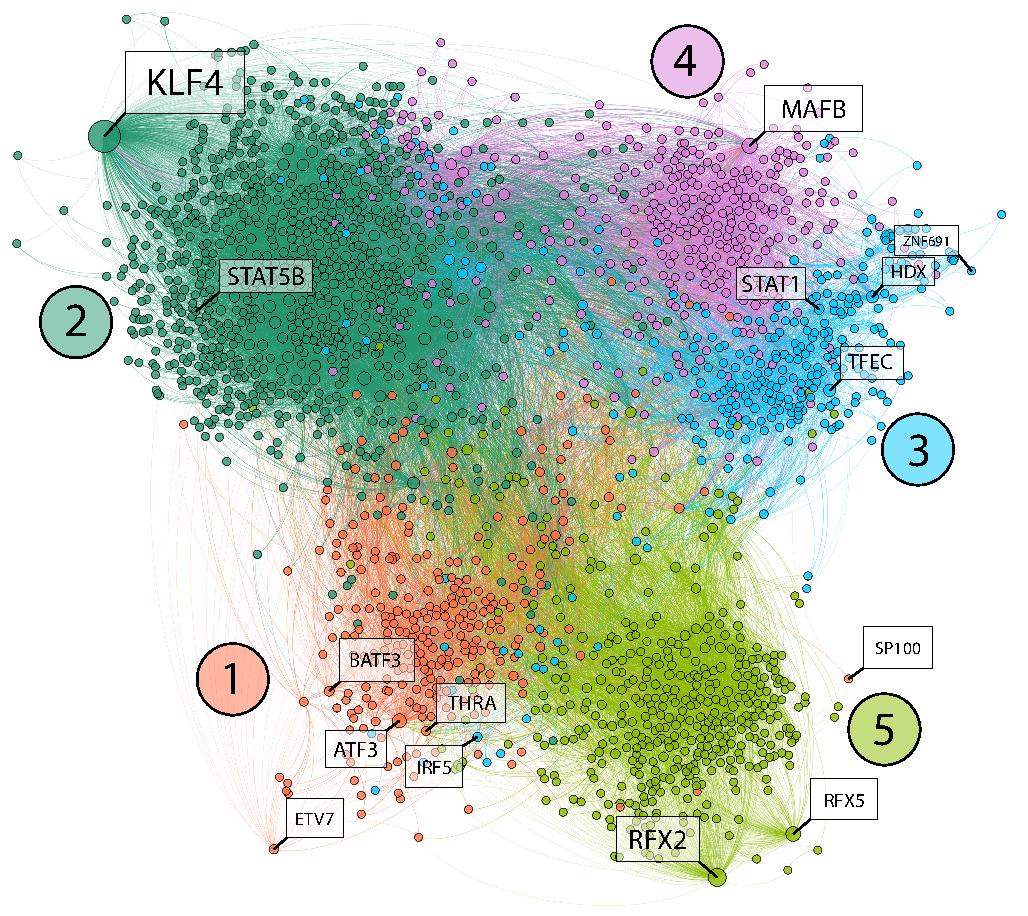
\includegraphics[width=\textwidth]{figures/cd14-ffl-modules}
\caption[Complete Feedforward Loop Network of Differentially Expressed Transcription Factors in CD14$^+$ Monocytes.]{\textbf{Complete Feedforward Loop Network of Differentially Expressed Transcription Factors in CD14$^+$ Monocytes.} Feedforward loops (FFLs) were created by \emph{miRNeo} query of transcriptional interaction of transcription factors (TFs), miRNAs, and tRFs towards all genes, but limited to FFLs of which the regulatory elements (TFs and smRNAs) were present and active in CD14$^+$ monocytes, and additionally filtered for the top 10\% TF$\to$gene relationships by activity. The resulting network was assembled in a force-directed 2D-projection and analysed to yield modularity information. The algorithm identified 5 distinct modules of small and large RNA FFLs, indicated by colours and numbers in circles. TFs differentially expressed in stroke patient blood are marked with a name tag (node size denotes differential expression count-change of TFs). 
\label{fig:cd14-ffl-modules}}
\end{figure}

\subsubsection{Module One}
GO enrichment analysis of significantly DE genes from module one resulted in 16 GO terms from 35 DE genes. The most significant biological process governed by module one is »negative regulation of transcription« with eight \acp{sg} and an adjusted p-value of \me{1.6}{4}. The second- and third-most significant terms indicate an influence on apoptotic processes (p = 0.0021 and 0.0049) with three \acp{sg}, which are a subset of genes from the first term, \emph{SP100}, \emph{SKIL}, and \emph{ATF3}. Further, module one genes are implicated in positive regulation of GTPase activity (5 SGs, p = 0.0069), epithelial cell differentiation (5 SGs, p = 0.0088), cellular response to IFN-$\upgamma$ (2 SGs, p = 0.024), platelet degranulation (2 SGs, p = 0.033), and cellular response to IL-1 (2 SGs, p = 0.049).

Apart from \emph{SP100} (major constituent of PML-SP100 bodies, see module three), \emph{SKIL} (part of SMAD pathway, regulating cell growth and differentiation), and \emph{ATF3} (member of the broadly acting CREB family of transcription factors), frequently implicated genes include \emph{CCL2} (chemokine ligand for CCR2, exhibits chemotactic activity for monocytes and basophils but not neutrophils and eosinophils pubmed 8627182,9792674,8195247) and \emph{CAMK1} (broadly acting calmodulin-dependent protein kinase, involved e.g. in the ERK cascade).

Module one genes, which decrease translational activity, are in the majority down-regulated, which may indicate a positive influence on transcriptional mechanisms, in line with the facilitation of a response to the insult. Given the uncertainty of whether the transcription factors of module one act as activators or repressors (FANTOM5 data only supplies binding probability, not mode of action), the real picture likely is more complicated, with mixed outcomes in expression regulation. A major component of module one processes is apoptotic signalling, which the top three (down-regulated) genes, \emph{SP100}, \emph{SKIL}, and \emph{ATF3}, are all involved in. All three genes are oncogenes, and as such involved in cell cycle control.

\emph{SP100} is induced by IFNs, presents with potent antiviral and tumour suppressor effects, and has been shown to induce apoptosis via the extrinsic pathway together with \emph{FLASH} or caspase-2 and p53 in \emph{PML} nuclear bodies (see module three).\cite{Sanchez-Pulido2007} A reduction of \emph{SP100} expression would thus likely lead to inhibition of apoptotic events. Histone deacetylase (\emph{HDAC}) inhibition (compare module five) suppresses the IFN-mediated \emph{SP100} up-regulation.\cite{Vlasakova2007} Recently, \emph{SP100}, \emph{STAT1} (compare module three), and \emph{KLF4} (compare module two) were found to be co-elevated in the peripheral monocytes of tobacco-smoking (but not in non-smoking) HIV-positive patients and associated with an increased depressive index.\cite{Lorenz2019}

\emph{SKIL}, also known as SnoN, is known as a pro-apoptotic mediator that can bind and activate p53, and is targeted by mir-30 family members, which can ameliorate its apoptotic effect.\cite{Kim2018} Conversely, Smad3, a pro-apoptotic protein, is repressed in synergy by \emph{STAT3} and the \emph{SKIL} paralog c-Ski.\cite{Makino2017} A recent study has identified \emph{SKIL} at the heart of a feedforward loop including \emph{EGR1} and hsa-miR-124-3p in the blood of schizophrenia patients, which showed a down-regulation of \emph{EGR1} and \emph{SKIL}, and concomitant up-regulation of miR-124-3p.\cite{Xu2016} However, in post-stroke whole blood, \emph{EGR1} and miR-124-3p are unchanged (own results).

\emph{ATF3} also shows a pro-apoptotic effect, as it can be activated by p38;\cite{Song2016} reduction of \emph{ATF3} in a cell model via siRNA interference reduced apoptosis.\cite{Sun2017} \emph{ATF3} is a key regulator of macrophage IFN responses, it represses pro-inflam"-ma"-to"-ry pathways (e.g. IL-6, TLR), and is also induced by IFNs. Correspondingly, \emph{ATF3}-deficient mice are more susceptible to endotoxin-mediated shock by cytokine overproduction. \emph{ATF3} and \emph{CXCL10} (compare module two) are co-induced by IFNs.\cite{Labzin2015} \emph{ATF3} sustains \emph{STAT3} phosphorylation through inhibition of phosphatases, and thus amplifies IL6-gp130-STAT3 signalling.\cite{Glal2018} \emph{ATF3} down-regulates \emph{ACHE} expression during stress by binding to the consensus recognition site of cyclic-AMP responsive element binding (CREB) proteins, »TGACGTCA«. In this case, a non-enzymatic, pro-apoptotic function of \emph{ACHE} is stipulated.\cite{Heinrich2018} Similarly, \emph{ATF3} attenuates hypoxia-induced apoptosis by down-regulating the expression of the pro-apoptotic factor carboxyl-terminal modulator protein (CTMP), via binding to the ATF/CREB site in the CTMP-promoter.\cite{Huang2015}

While module one genes present a complex regulatory picture, the function of the three most-involved genes may be summarised as pro-apoptotic; their consistent down-regulation in patient blood after stroke thus implies an inhibition of apoptotic processes inside module one. Additionally, \emph{SP100} and \emph{ATF3} present with clear ties to cholinergic processes, in their involvement with neurokines and STATs, association with nicotine consumption, and the attenuation of \emph{ACHE} expression. 

\subsubsection{Module Two}
Module two, being the largest module, predictably also offers most process-related terms (50 GO terms, 34 SGs), of which most are related to immunity or basic processes of cell physiology. For the sake of clarity, immunity terms will be explored first. Module two genes most significantly participate in regulation of response to cytokine stimulus (4 SGs, p = \me{2.9}{4}), response to LPS (5 SGs, p = \me{5.6}{4}), inflammatory response (6 SGs, p = 0.0015), and T- and B-cell differentiation (2 SGs each, p = 0.036 and 0.041). The highest DE genes from module two involved in these processes are \emph{SORL1} (a known regulator of neurokine signalling), \emph{STAT5B}, the IL-10 receptor $\upalpha$, \emph{PLXNB2} (involved in cell migration),  \emph{JAK2}, the transcription factor \emph{KLF4} (with many broad functions, but implicated in MAPK/ERK cascades and IL-4 mediated macrophage differentiation\cite{Ghaleb2017}), \emph{PTPN2} (phosphatase involved in dephosphorylating JAKs and STATs), and \emph{CXCL10} (pro-inflammatory chemokine ligand implicated in response to brain injury by activating microglia).
 
Non-immune physiological terms refer to regulation of cell migration (8 SGs, p = \me{1.4}{4}), negative regulation of MAPK cascade (4 SGs, p = \me{4.7}{4}), cellular response to peptide (5 SGs, p = \me{9.5}{4}), nucleus organisation (3 SGs, p = 0.0010), erythrocyte differentiation (3 SGs, p = 0.0010), negative regulation of cell adhesion (4 SGs, p = 0.0015), regulation of ERK cascade (3 SGs, p = 0.0085), regulation of angiogenesis (3 SGs, p = 0.013), regulation of cold-induced thermogenesis (2 SGs, p = 0.031) and several more basic processes. Many of these processes appear to be vital to the immune functions described above, as they share many of the most highly DE genes, such as \emph{SORL1}, \emph{STAT5B}, \emph{PLXNB4}, \emph{KLF4}, and \emph{PTPN2}. 

Module two includes several genes directly involved in the JAK/STAT immune response, such as \emph{IL10RA}, \emph{JAK2}, \emph{STAT5B}, and \emph{PTPN2}; module two genes are mostly down-regulated except for \emph{SORL1} (which shows dramatic increase in terms of count-change) and \emph{STAT5B}.

\emph{SORL1} gives rise to the protein SorLA, synonymous with LR11, a transmembrane receptor that can interact with a wide variety of ligands intra- as well as extra-cellularly.\cite{Yin2015} SorLA is primarily known as the neuronal ApoE4 receptor, and thus widely associated with AD risk. Among other functions, it regulates APP trafficking and processing, and is significantly decreased in the AD-vulnerable regions of late-onset AD patients.\cite{Yin2015} However, in addition to its well-studied neuronal roles, it is highly expressed on the surface of monocytes and macrophages, and additionally up-regulated in acute myeloic leukaemia.\cite{Sakai2012} SORL1 binds many immune-related ligands such as the neurokine IL-6 and soluble neurokine receptors IL6R and CNTFR, mediating their cellular uptake. It associates with the transmembrane IL-6 receptor and reduces downstream effects via a reduction in STAT3 phosphorylation.\cite{Larsen2017} Conversely, while decreasing \emph{cis} signalling as just described, SORL1 may increase \emph{trans} signalling, i.e., IL6 availability in the blood stream which then binds to the soluble IL6 receptor and can affect any cell possessing the ubiquitously distributed gp130.\cite{Rabe2008} It has been shown that overexpression of a soluble gp130 form can effectively suppress inflammation mediated by the soluble IL6 receptor without interfering with the function of the transmembrane IL6 receptor.\cite{Rabe2008}

\emph{PLXNB2} can promote inflammation via activation of the NF-$\upkappa$B pathway.\cite{Zhang2018} In addition, it prominently mediates a plethora of the functions of angiogenin (ANG): it is the receptor for ANG in physiological and pathological cells; ANG acts though \emph{PLXNB2} on cell proliferation; \emph{PLXNB2} modifies ANG RNA-processing activity and cell type specificity (see Section \ref{sec:intro:trfs}); and \emph{PLXNB2} mediates neuroprotective effects of ANG.\cite{Yu2017} A recent study shows its close association to inflammation-related circulatory events: upon inflammatory stimulation (using TNF-$\upalpha$, IL-1$\upbeta$, IL-4, and IL-6) of murine and human cells, endothelium-derived extracellular vesicles carrying miRNAs were released and taken up by monocytes causing decreased monocytic \emph{PLXNB2} levels and increased splenic monocyte mobilisation.\cite{Akbar2017} Twelve miRNAs were enriched in these vesicles, which show high similarity to differential expression in stroke patient blood (own results in brackets); these are hsa-miRs: -632 (not detected in stroke), -126-3p (\ac{lfc} = -1.12, p = \me{3.0}{11}), 151a-3p (\ac{lfc} = -2.37, p = \me{5.6}{22}), -26b-5p (\ac{lfc} = -1.17, p = \me{5.0}{5}), -126-5p (\ac{lfc} = -2.23, p = \me{5.2}{7}), -7a-5p (\ac{lfc} = -0.54, p = 0.03), -1972 (not detected), -15b-5p (\ac{lfc} = -0.85, p = \me{5.2}{7}), -23a-3p (\ac{lfc} = -1.68, p = \me{9.9}{16}), -374b-5p (\ac{lfc} = -1.85, p = \me{1.3}{5}), -23b-3p (\ac{lfc} = -1.73, p = \me{1.2}{17}), and -7b-5p (\ac{lfc} = 0.73, p = \me{4.1}{6}). In another study, \emph{PLXNB2}-deficient macrophages showed greater mobility and would healing capabilities than WT cells.\cite{Roney2011}

\emph{KLF4} has gained much attention since it was discovered to be one of the four factors for induction of pluripotent stem cells (iPSCs, induced by Oct3/4, Sox2, Myc, and Klf4).\cite{Takahashi2006} In macrophages (often using the model RAW264.7), \emph{KLF4} controls activation in response to LPS stimulation by regulating, among others, NF-$\upkappa$B, TGF-$\upbeta$, IL-1$\upbeta$, and HMGB1, at least partly through Smad3 inhibition (compare module one).\cite{Feinberg2005,Liu2008,Liu2012} In monocytes, \emph{KLF4} regulates differentiation towards a pro-inflammatory type of resident monocytes, such that \emph{KLF4} KO mice completely lacked inflammatory monocytes in blood and spleen.\cite{Feinberg2007,Alder2008,Kurotaki2013}
%interacts with sumo (sp100, pml)

The protein tyrosine phosphatase \emph{PTPN2} is implied in IL-1$\upbeta$-mediated inflammation. Mice deficient of \emph{PTPN2} die few weeks after birth because of anaemia, colitis, and severe systemic inflammation. Macrophages depleted of \emph{PTPN2} show excessive inflammasome activation. \emph{PTPN2} reduction leads to more general inflammation, but also less tumour susceptibility, likely because of a more efficient eradication of oncogenic cells.\cite{Spalinger2018} Increased inflammatory cascades following \emph{PTPN2} reduction are likely caused by the decrease in \emph{STAT1} and \emph{STAT3} dephosphorylation, and the concomitant increase in STAT signalling (compare module five, \emph{HDAC7}).\cite{Kim2018a}
 
In summary, module two genes seem to be responsible for facilitating an adequate immune response by regulating basic processes in order to enable immune cells to fulfil their functions (e.g., response to cytokines and cellular mobility). Since most of module two genes are down-regulated in stroke patient blood, the summative effects are likely immuno-suppressive, which is in concordance with down-regulation of the LPS response pathway genes. MAPK? \todo{}

\subsubsection{Module Three}
Module three, with 14 GO terms and 13 SGs, appears similar in principle to module two, although much fewer basic physiological terms are involved. This is explained by the smaller size of the test set; the ontologies for basic terms include substantially more genes, and the likelihood of significant enrichment in the test set is reciprocal to test set size. The most significant biological processes of module two genes involve cellular response to IFN-$\upgamma$ (3 SGs, p = \me{1.6}{4}) and positive regulation of transcription (5 SGs, p = \me{9.1}{4}), as opposed to negative regulation of transcription found in module one. Further, module three genes are involved in the cytokine-mediated signalling pathway (4 SGs, p = 0.0018), regulation of IFN production (2 SGs, p = 0.0034), JAK-STAT cascade (2 SGs, p = 0.0048), negative regulation of angiogenesis (2 SGs, p = 0.0056), regulation of innate immune response (2 SGs, p = 0.035), and positive regulation of cytokine production (2 SGs, p = 0.048). Most frequently occurring genes are \emph{STAT1}, \emph{PLSCR1} (implicated in amplification of IFN response), \emph{PML} (also associated with IFN- and TNF-responses), and \emph{IRF5} (implicated in TLR7/8-induced induction of IFNs and other pro-inflammatory cytokines).

Phospholipid scramblase 1 (\emph{PLSCR1}) is an oncogene implicated in cell cycle control, apoptosis, and mediation of antiviral response. While its mechanism of action is yet unexplained, the mature protein localises to the nucleus and has been shown to bind DNA.\cite{Ben-Efraim2004} While it does not induce apoptosis on its own, its overexpression has inhibitory effects on several cell cycle controllers and anti-apoptotic proteins such as Bcl-2.\cite{Huang2006} \emph{PLSCR1} participates in the antiviral response by potentiating IFN activity, which increases expression of a subset of \acp{isg}, including STAT1.\cite{Dong2004} It is expressed in human macrophages and monocytes, in which it is increased in systemic inflammatory conditions, and seems to also contribute to pro-thrombotic conditions.\cite{Suzuki2010,Herate2016} 

Promyelocytic leukaemia protein (\emph{PML}) is, together with \emph{SP100} (see module one), the major constituent of PML nuclear bodies, that are also known as \ac{nd10}. These small nuclear organelles are known for their peculiar and enigmatic function in antiviral response, which they seem to convey by a wide variety of molecular functions, from chromatin modification to physical trapping of virus particles.\cite{} Recently, however, they have also been connected to a direct regulation of innate immune responses. IFN therapy increases the expression of both \emph{PML} and \emph{SP100}, and enhances their antiviral activity.\cite{Regad2001} Correspondingly, \emph{PML} depletion reduces the capacity of IFNs to interfere with viral infection.\cite{Chee2003} PML has the capacity to modulate different stages of the pathway from IFNs through ISGs to the activation of STATs by associating with and stabilising transcription factor complexes, for instance by binding directly to \emph{STAT1} and \acp{irf} (see below).\cite{Chen2015} The production of IL-1$\upbeta$ and IL-6 is significantly reduced in \emph{PML}-deficient cells;\cite{Lo2013} and correspondingly, \emph{PML}-deficient mice are resistant to LPS-mediated lethality.\cite{Lunardi2011} This directly links to an epigenetic switch that leads to cellular transformation: inflammation, through NF-$\upkappa$B, activates Lin28 and rapidly reduces let-7 miRNA levels. This leads to de-repression of the IL-6 mRNA, and the increased IL-6 peptide conveys cellular transformation through \emph{STAT3} activation, as well as positive feedback by inducing NF-$\upkappa$B synthesis.\cite{Iliopoulos2009}

\emph{IRF5}, a well-studied member of the Interferon Regulatory Factor transcription factor family, is an important element of most blood-borne immune cell types, particularly of macrophages and pro-inflammatory monocytes.\cite{Li2016} It has been demonstrated that \emph{IRF5} is involved in transcriptional induction of IL-6, IL-12, and TNF-$\upalpha$ mediated by the \acf{tlr}/\ac{myd88} complex. \emph{IRF5}-deficient mice also show resistance to LPS-mediated lethality (compare PML/SP100).\cite{Takaoka2005} While KO-mice showed severely impaired production of the aforementioned cytokines, IFN-$\upalpha$ production was not impaired; the responsible interferon-stimulated response elements have yet to be determined.\cite{Takaoka2005} \emph{IRF5} is highly expressed in monocytes and macrophages as well as B cells and dendritic cells, and its expression is induced by a pro-inflam"-ma"-to"-ry environment.\cite{Krausgruber2011} On the spectrum of macrophage state after differentiation, \emph{IRF5} (together with \emph{IRF1} and \emph{IRF8}) is involved in the commitment to a pro-inflammatory (M1) phenotype (as opposed to the »wound healing« M2 type).\cite{Chistiakov2018}  The M1 phenotype is brought about by increased activity of NF-$\upkappa$B and STAT1, whereas the M2 counterpart is induced by IL-4-, IL-10-, and IL-13-mediated STAT3 and STAT6 signalling.\cite{Wang2014a} Molecular competition for MyD88 binding between IRF5 and IRF4 is crucial for the determination of pro- (\emph{IRF5}) or anti-inflammatory (\emph{IRF4}) differentiation.\cite{Negishi2006} Thus, a down-regulation of IRF5 together with unchanged levels of IRF4, as is the case in stroke patient blood (own results), would lead to anti-inflammatory conditions in monocyte and macrophage populations. M1$\to$M2 macrophage transition supports resolution of inflammation and tissue healing, and modulation of IRF5 expression in monocytes and macrophages via siRNA interference improved healing after cardial infarcts and skin wounds in mice, in parallel with a reduction in pro-inflammatory cytokines IL-1$\upbeta$, IL-6, and TNF-$\upalpha$.\cite{Courties2014}

Visually (in the two-dimensional force-directed map), module three is the module most »intermingling« with the other modules, particularly in the case of \emph{IRF5}, which spatially is closer to module one and five than it is to three (see Figure \ref{fig:cd14-ffl-modules}, bottom). More generally, there are two zones of module three intermingling, between modules one and five, and between modules two and four. In the t-SNE visualisation of GO terms, module three terms cluster on the left side in close vicinity of the central cluster around module one terms.

Module three genes (implicated in positive regulation of transcription, but all down-regulated) appear to act in partial opposition to module one genes (implicated in negative regulation of transcription, and all down-regulated), thus possibly being part of homeostatic events surrounding gene transcription in response to inflammatory events. Module one and three share GO terms involved in responses to, and production of, interferons and interleukins.

In summary, module three seems to be representative of immune suppression via several mechanisms; mediation of pro-inflammatory signalling via INFs is repressed, and IRF5 suppression may induce an anti-inflammatory, pro-resolving differentiation of monocytes and macrophages; cytokines and STAT signalling are likewise down-regulated; ND10 nuclear bodies are repressed. On the other hand, pro-apoptotic signalling might be de-repressed via PLSCR1 reduction. 

\subsubsection{Module Four}
Module four, with 12 significant GO terms from 7 SGs, is a fairly small module, which is nevertheless highly associated with immune processes; most significantly, genes of module four convey positive regulation of innate immune response (2 SGs, p = 0.0039) and positive regulation of cytokine production (2 SGs, p = 0.0075); more accurately, IL-1 production (1 SG, p = 0.038). Further, module four genes show association with negative regulation of myeloid cell differentiation (1 SG, p = 0.038), positive regulation of response to cytokine (1 SG, p = 0.038), myeloid cell homeostasis (1 SG, p = 0.042), positive regulation of inflammatory response (1 SG, p = 0.045), and negative regulation of myeloid leukocyte differentiation (1 SG, p = 0.049). The most prevalent SGs in these terms are \emph{GBP5} (activator of the NLRP3 inflammasome assembly), \emph{MAFB} (transcription factor required for monocyte differentiation), and \emph{ZBP1} (cytoplasmic DNA-sensor which activates downstream IFN production in activated macrophages).

\emph{GBP5} (for Guanine Nucleotide Binding Protein) is a molecular marker for the classically activated, pro-inflammatory M1 type macrophage,\cite{Fujiwara2016} and a critical factor for the assembly of the \emph{NLRP3} inflammasome.\cite{Shenoy2012} \emph{GBP5} is strongly induced by IFNs through NF-$\upkappa$B, and in turn induces expression of IFNs and pro-inflammatory cytokines such as IL-6 and TNF-$\upalpha$.\cite{Feng2017} Consequentially, it plays a critical role in response to viral infection, e.g. by Influenza or HIV, as well as diverse other pathogens.\cite{Feng2017,Krapp2016} In mice, miR-21-5p inhibition led to an increase in macrophage GBP5, with a concomitant increase in TNF-$\upalpha$ and a decrease in the anti-inflammatory IL-10.\cite{Corsetti2018} However, in stroke patient blood, both miR-21-5p and GBP are down-regulated (own results).

\emph{MAFB} is a transcription factor with critical roles in macrophage differentiation and function, and specific for mononuclear phagocytes in all cells of the hematopoietic system.\cite{Hamada2020} Macrophages deficient in \emph{MAFB} and \emph{MAF} reacquire the ability for self-renewal, but only upon concomitant up-regulation of two pluripotent stem cell-inducing factors, \emph{KLF4} and \emph{MYC} (compare module two).\cite{Aziz2009} However, in stroke patient blood (own results), \emph{KLF4} is reduced while \emph{MAF} and \emph{MYC} are unchanged. After induction of ischemic stroke, macrophage-specific \emph{MAFB}-deficient mice showed excessive sterile inflammation, likely due to a failure in clearing of \acp{damp}.\cite{Shichita2017} The authors found \emph{MAFB} to be a critical controller of the macrophage scavenger receptor 1 (MSR1), which in turn is essential for the clearance of DAMPs after ischemic stroke, and is also down-regulated in stroke patient blood (own results, \ac{lfc} = -3.54, p = \me{2.9}{6}). Additionally, retinoic acid receptor agonist \emph{Am80} increased \emph{MAFB} and \emph{MSR1} expression in the delayed phase of ischemic stroke, and had ameliorating effects on stroke pathology.\cite{Shichita2017} \emph{miRNeo} query of retinoic acid receptor interactions in CD14$^+$ cells indicates \emph{RARA}, the $\upalpha$ retinoic receptor, as most active towards MAFB (lower activity also exhibited by \emph{RARG} and \emph{RXRA}). \emph{RARA} also targets STATs 1, 5A, and 5B, as well as \emph{ACHE} and \emph{IL6ST} (also known as gp130) in these cells. 

An \emph{ex vivo} experiment of \emph{MAFB} inhibition by siRNA in human CD14$^+$ monocytes found an elevation in IRF3 phosphorylation and concomitant increase in INF-$\upalpha$ and INF-$\upbeta$ production.\cite{Liu2019} \emph{MAFB} also seems responsible for direct regulation of all genes of the C1q complement complex, which activates the classical component pathway.\cite{Tran2017} Thereby, and by regulation of the Axl protein, \emph{MAFB} is essential for efferocytosis, the phagocytosis of apoptotic cells \emph{in vivo}.\cite{Sato2018} \emph{MAFB} is regulated by diverse pathways; immunological mediators (e.g. cytokines), lipid metabolism, and miRNAs.\cite{Hamada2020} Two miRNAs experimentally identified as regulating \emph{MAFB}, miR-152\cite{Tozaki-Saitoh2019} and miR-155\cite{Jablonski2016}, are significantly down-regulated in stroke patient blood (own results; hsa-miR-152-3p: \ac{lfc} = -1.97, p = \me{2.0}{11}; hsa-miR-155-5p: \ac{lfc} = -0.69, p = \me{6.5}{4}). miR-155 has additionally been shown to induce pro-inflammatory macrophages, while \emph{MAFB} itself promotes anti-inflammatory M2-type macrophage differentiation.\cite{Kim2017} In CD14$^+$ monocytes, MAFB interacts with \emph{CHRNA6}, \emph{IL6}, the \emph{IL6R} receptor, and \emph{STAT1} (via \emph{miRNeo}, from Marbach \emph{et al.} regulatory circuits\cite{Marbach2016}). In summary, \emph{MAFB} reduction after stroke might contribute to a shift towards pro-inflam"-ma"-to"-ry M1\-/type macro"-phages, prolonged activity of which might inhibit efferocytosis and the M2-mediated healing process in the delayed phase.

Z-DNA binding protein 1 (\emph{ZBP1}, also known as \emph{DAI}) is an IFN-induced cytoplasmic sensor of \acp{damp} that positively mediates various forms of programmed cell death, general pro-inflammatory events (such as cytokine production), and \emph{NLRP3} inflammasome assembly; however, its triggering ligands or molecular patterns are still unclear.\cite{Kuriakose2018} More recently, it was shown that \emph{ZBP1} is necessary for type-I and type-II IFN-mediated necroptosis (a programmed form of necrosis),\cite{Yang2019} by sensing viral as well as endogenous RNA (in addition to DNA), possibly in the unusual Z-conformation.\cite{Maelfait2017} Murine macrophages lacking the \ac{myd88} TLR adapter protein were able to undergo apoptosis through redundant TLR pathways mediated by \emph{ZBP1}. In contrast, KO of the type-I INF receptor, as well as of its downstream effectors \emph{STAT1} and \emph{IRF9}, abolished the macrophages' ability to undergo TLR-mediated \ac{myd88}-independent apoptosis.\cite{Kuriakose2016} Moreover, de-novo transcription and protein synthesis (compare »regulation of transcription« in modules one and three), as well as JAK1/STAT1 transcriptional activation are required for IFN-induced necroptosis through \emph{ZBP1} signalling.\cite{Yang2019} \emph{ZBP1}-deficient mice (via CRISPR/Cas-9 KO) were significantly protected from acute IFN-mediated \acf{sirs},\cite{Yang2019} making the \emph{ZBP1} down-regulation in stroke patient blood (own results, \ac{lfc} = -1.70, p = 0.001) a logical bodily response to prevent \acf{cids}, and a possible component of the counter-regulation, \acf{cars} (see Section \ref{sec:intro:stroke}). Notably, NF-$\upkappa$B signalling blocks type-II IFN-induced necroptosis (compare modules two and three).\cite{Thapa2011}

%homointeraction and RIPK3 interaction of ZBP1?

In summary, module four constitutes a small, largely anti-inflammatory module, conveying an attenuation of inflammatory processes by limiting the sensing of inflammatory stimuli (\emph{ZBP1}), activation of inflammatory pathways, inflammasome assembly and cytokine production (\emph{GBP5}), and clearance of DAMPs in the infarct area (\emph{MAFB}). However, the decrease in \emph{MAFB} expression may also promote a delayed phenotypic shift towards M1-type macrophages, which may have a deleterious effect on patient recovery.

\subsubsection{Module Five}
Module five is a medium-sized module (29 GO terms from 18 SGs) which is only loosely associated with immunity. Most terms relate to basic molecular functions of the cell, such as regulation of cell-substrate adhesion (3 SGs, p = 0.0037), cellular component maintenance (2 SGs, p = 0.0052), membrane depolarisation (2 SGs, p = 0.0052), regulation of protein tyrosine kinase activation (2 SGs, p = 0.0063), positive regulation of small molecule metabolism (2 SGs, p = 0.0063), fatty acid metabolic process (3 SGs, p = 0.0064), positive regulation of lipid metabolic process (2 SGs, p = 0.010), regulation of cytokine production (3 SGs, p = 0.022), response to hypoxia (2 SGs, p = 0.027), and several more. The genes most highly implicated in these processes are \emph{SRC} (tyrosine kinase activated by immune response receptors, that facilitates immune response, adhesion and migration, and apoptosis), \emph{ABCD1} (ATP-binding cassette transporter for very-long-chain fatty acids, implicated in regulation of inflammatory response by positively regulating peroxisomal beta-oxidation), and \emph{HDAC7} (histone deacetylase with inflammatory implications).

Src, from the \emph{SRC} gene, is a well-studied kinase from the larger family of Src kinases implicated in diverse physiological processes. Increased \acf{vp}, i.e., a loss of blood-brain-barrier function, can be induced by TNF-$\upalpha$, IL-1$\upbeta$, IL-6, and \ac{vegf}. Src family kinases can physically bind to gp130, phosphorylate STAT3,\cite{Brown1996} and are intricately involved with TLR-CD14 signalling, in an important but not obligatory manner.\cite{Okutani2006} Of relevance, Src controls \ac{vegf} expression after ischemic stroke, thereby modulating \ac{vp}. Reduction of Src (but not Src family kinase Fyn) activity in mice via complete congenital KO or pharmacologic inhibition (using the synthetic inhibitor PP1) resulted in a reduction of permanent \ac{mcao}-induced stroke volume of 50\% and up to 70\%, respectively. This beneficial effect was associated with a prevention of \ac{vp}.\cite{Paul2001} In these experiments, Src inhibition seemed to restore perfusion and oxygenation in the penumbra (the region adjacent to the infarct), protecting the surrounding tissue. Later, these VEGF-modulating effects of Src on \ac{vp} and stroke recovery were replicated in rats with transient infarction.\cite{Zan2014} In another set of experiments, it was shown that the neuroprotective effect of ischemic postconditioning in mice probably depends in Src kinase activation.\cite{Kumar2014b} In a human cellular model, Src was up-regulated upon inflammatory TNF-$\upalpha$ signalling and conveyed increases in \ac{vp} in a p38 MAPK-dependent manner.\cite{Adam2016} 

\emph{ABCD1} is a member of the \ac{abc} superfamily of active transporters, responsible for the transport of very long chain fatty acids.\cite{Hama2018} It is best known for its role in \ac{ald}, where an \emph{ABCD1} deficiency leads to microvascular perfusion anomalies in the brain.\cite{Lauer2017} The working hypothesis states that \emph{ABCD1}-related up-regulation of adhesion molecules in the endothelium causes higher leukocyte interaction and thus impairs blood flow in the capillaries. Notably, carriers of the ApoE4 allele are more significantly affected by \ac{ald}.\cite{Orchard2019} Most molecular changes caused by the deficiency are likely a result of impaired fatty acid transport into peroxisomes. \emph{Abcd1}-deficient mice show a dramatically altered brain region-specific phospholipid profile.\cite{Hama2018}

\emph{HDAC7} (histone deacetylase 7) is a protein responsible for deacetylating histones and non-histone proteins, with regulatory implications in cell proliferation, apoptosis, differentiation, and migration.\cite{Lei2017} \emph{Hdac7}$^{-/-}$ mice are embryonic lethal because of an angiogenetic failure leading to rupture of blood vessels.\cite{Chang2006} It has been shown that \emph{HDAC7} directly interacts with \emph{STAT3}, deacetylation of which interferes with its ability to dimerise, thus impairing its functionality.\cite{Peixoto2016,Lei2017} \emph{HDAC7} was also found to induce an apoptotic gene program and c-Myc suppression upon ectopic expression in human SD-1 cells.\cite{Barneda-Zahonero2015} \emph{HDAC7} additionally suppresses macrophage genes relevant for phagocytosis, TLRs, interleukins and TNF pathway genes by acting as a transcriptional repressor of myocyte enhancer factor \emph{MEF2C}.\cite{Barneda-Zahonero2013} In human C10 cells reprogrammed to macrophages, \emph{HDAC7} expression significantly inhibited the expression of TNF-$\upalpha$, IL-1$\upbeta$, and IL-6.\cite{Barneda-Zahonero2013} VEGF stimulates HDAC7 phosphorylation, leading to its aggregation in the cytosol and subsequent suppression of angiogenesis mediated by matrix metalloproteases (MMT) 10 and 14, which degrade proteins essential for vessel integrity.\cite{Miano2006,Ha2008} \emph{HDAC7} can also directly associate with \emph{RARA} (see module four, \emph{MAFB}) to form a repressor complex that inhibits, among others, miR-10a.\cite{Lee2017} This inhibition led to de-repression of pro-inflammatory signalling via \emph{GATA6} and \emph{VCAM1}, with negative impact on \ac{vp} in vascular endothelia.
 
The only module in which directions of expression in most GO terms are mixed, general implications, broad spectrum, metabolic aspect, spatially close to module one?

positive lipid metabolic: SRC and ABCD1, both down -> metabolism brake
HDAC7 up -> pro-apoptotic

\subsubsection{Module Summary}
modules represent changes brought on by DE TFs in stroke blood, focused on CD14 by definition of feedforward loop smRNAs presence and TF-interactions specific to CD14

modules one and five do not mix with modules two and four, three is »in the middle«

one and three antagonism/homeostasis?

most prevalent genes identified by module go are pivotal regulators of immunity

the relevant genes identified are involved in 3.5\% of miRNA FFLs (681 FFLs) and 11\% of tRF FFLs (21 FFLs)

small network of above genes?

\subsection{Transcript Clustering by smRNA:TF:gene Feedforward Loops Increases Informative Resolution of Gene Set Enrichment Analyses}

central cluster - cooperative zone? genes involved?

mRNA down, tRF up, miRNA down -> miRNA-like tRF function coherent, miRNAs in general incoherent, displacement tRF mechanism also incoherent. but, few FFLs in miRNA-like tRFs. fig \ref{fig:stroke-de-tsne}

\begin{figure}
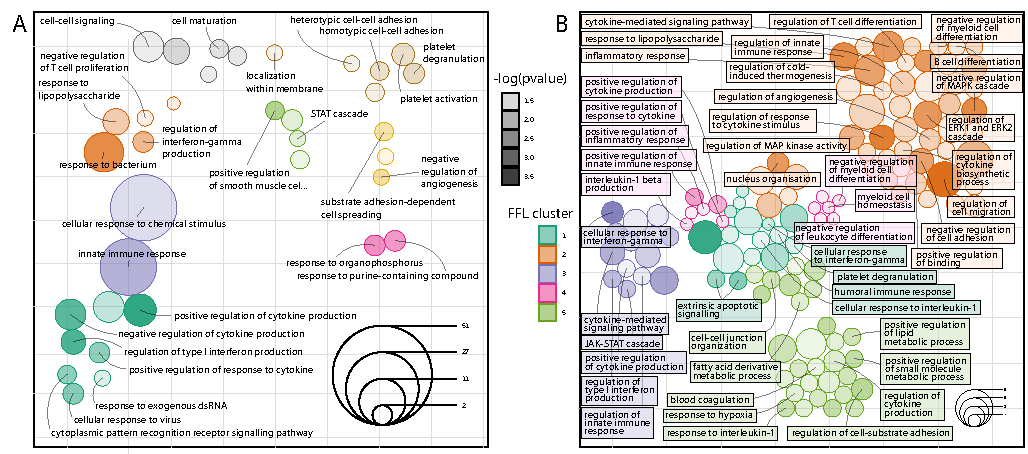
\includegraphics[width=\textwidth]{figures/gsoap-ffl}
\caption[FFL module Gene Ontology Enrichment.]{\textbf{FFL module Gene Ontology Enrichment Increases Informative Resolution.} A comparison between GO enrichment performed on (A) differentially expressed (DE) genes and (B) DE genes classified by FFL network modules shows similar biological processes but increased information depth. Size denotes number of significant genes in term, colour indicates p-value (all p < 0.05). \textbf{A)} DE genes with absolute ac{lfc} > 1.4 are enriched in processes of immunity and circulation. Cluster colour derived from t-SNE similarity. Reproduction of Figure \ref{fig:gsoap-de}. \textbf{B)} t-SNE mapping of GO terms derived from analysis of single FFL modules shows details of involvement with immune processes and basic cellular function. Colour indicates original FFL module (see text). The middle cluster, comprised of parts from all modules surrounding module 1, may signify an »area of cooperation« between the modules.
\label{fig:gsoap-ffl}}
\end{figure}

%
%\section{Dimensionality Reduction and Correlation of Expression with Clinical Parameters}
%
%\begin{method}
%
%\subsection{WGCNA}
%Reduction of dimensionality of high-dimensional data, such as the expression of thousands of small RNA species and their correlation with clinical parameters of patients, can also be achieved by means of Weighted Gene Correlation Network Analysis (WGCNA, also R/WGCNA).\cite{Langfelder2008} The aim of this method is the identification of modules that group similarly-expressed genes. Each of these modules is represented by an eigenvector (called \emph{eigengene}), effectively replacing the individual expression parameters of the genes in the module. The eigengene can then be used to determine correlation of covariates to each module.
%
%To represent expression data in a network-based manner, the expression matrix is transformed into an adjacency matrix representing similarities between nodes, i.e., genes. The co-expression similarity $s_{ij}$ between two nodes $i$ and $j$ is defined as the absolute correlation coefficient between the expression profiles $$s_{ij} = |cor(x_i, x_j)|$$ with $x$ representing the node expression profile. A signed co-expression measure can be used to keep track of the direction of co-expression. Weighted networks allow the adjacency measures to assume continuous values between 0 and 1, thereby retaining the continuous nature of the underlying expression matrix. This is achieved by implementation of a soft threshold, which is usually chosen by the user to result in a scale-free network topology. The connectivity distribution in a scale-free network follows a power law, i.e., the probability of a node with $k$ connections is, for large values of $k$: $$P(k) = k^{-\alpha}$$ With $\alpha$ usually between 2 and 3. Many biological networks are assumed to be scale-free; however, this assumption has very recently been empirically questioned.\cite{Broido2019}
%
%Once the network is created, modules are identified via unsupervised clustering of densely connected nodes. Biological significance can then be assigned to each of the modules and genes. Module eigengenes can be calculated (the first principal component of the module) and correlated to traits, such as clinical parameters. In this manner, modules with potential functional implications can be identified.
%
%\subsection{Co-correlation}
%The fact that a subset of small \ac{seq} samples were also subjected to large \ac{seq} enables the application of a secondary correlation between those two approaches. For instance, module eigengenes derived from \ac{smrna} analysis can be correlated with the mRNA module eigengenes across the common patients. The module similarity $\sigma$ thus is defined as the correlation coefficient between eigengene profiles $e$ of modules $i$ and $j$: $$\sigma = |cor(e_i, e_j)|$$
%
%Significantly correlating modules (p < 0.05) were identified and further analysed downstream.
%
%%\section{Direct Interaction}
%
%\end{method}
%
%


